\documentclass{report}

%Packages pour les langues
\usepackage[utf8]{inputenc}
\usepackage[T1]{fontenc}
\usepackage[french]{babel}
\usepackage{lmodern}

%Package pour la mise en forme (marges)
\usepackage[a4paper]{geometry}
\geometry{hscale=0.85,vscale=0.85,centering}
\usepackage{layouts} %affichage des largeurs de zone texte
\usepackage{parallel}
\usepackage{setspace}
\usepackage{wrapfig}
%Packages pour les liens dynamiques
\usepackage{hyperref}
\usepackage{multicol}
%\usepackage{underscore}

%Packages pour les formules de Maths
\usepackage{amsmath}
\usepackage{amssymb}
\usepackage{mathrsfs}
\usepackage{mathtools}
\usepackage{pseudocode}
\usepackage{fancybox}

%Packages des images
\usepackage{graphicx}
%\usepackage{pdftricks}
%\begin{psinputs}
%   \usepackage{pstricks}
%   \usepackage{multido}
%\end{psinputs}

%\usepackage{subfigure}
\usepackage{subfig}
\usepackage{wrapfig}
\usepackage{caption}

%\usepackage{subcaption}
\usepackage{float}

%Packages pour le glossaire
\usepackage{glossaries}

%\usepackage[xindy]{glossaries}
\makeglossaries

%Package pour colorier le code Matlab (copyright Jérémy Fauvel)
\usepackage{listings}
\usepackage[usenames,dvipsnames]{color}

%Code pour afficher du code Matlab
\definecolor{MyDarkGreen}{rgb}{0.0,0.4,0.0}
\lstset{language=Matlab, frame=none, basicstyle=\small\ttfamily, keywordstyle=[1]\color{Blue}\bfseries, keywordstyle=[2]\color{Purple}, keywordstyle=[3]\color{Blue}\underbar, identifierstyle=, commentstyle=\usefont{T1}{pcr}{m}{sl}\color{MyDarkGreen}\small, stringstyle=\color{Purple}, showstringspaces=false, tabsize=5, morekeywords={xlim,ylim,var,alpha,factorial,poissrnd,normpdf,normcdf}, morekeywords=[2]{on, off, interp}, morekeywords=[3]{FindESS, homework_example}, morecomment=[l][\color{Blue}]{...}, numbers=left, firstnumber=1, numberstyle=\tiny\color{Red}, stepnumber=1}

%Packages pour les string
\usepackage{xstring}

%Packages pour les listes
%\usepackage{enumitem}

\begin{document}
\begin{titlepage}
\title{Rapport de stage - IRR \\ Implémentation et application d'un algorithme dynamique hybride pour le contrôle d'articulations flexibles}
\date{3 Mars 2014 - 31 Août 2014}
\author{Auteur: \bsc{Guedelha} Nuno \\ Tuteur: \bsc{Stasse} Olivier}
\end{titlepage}

\setcounter{secnumdepth}{3}

\graphicspath{{illustrations/}}
\maketitle

%Rennomer la table des matières en Sommaire
\renewcommand{\contentsname}{Sommaire}
\tableofcontents
\listoffigures
\listoftables

%%%%%%%%%%%%%%%%%% Macros %%%%%%%%%%%%%%%%%%%%%%%%%%%%%%%

%=============== variable fichier de figures ==============================

\newcommand{\myFiguresFile}{}
\newcommand{\setmyFiguresFile}[1]{\renewcommand{\myFiguresFile}{#1}}

%=============== include 1 figure =========================================

\ifx \incFig \undefined
\def \incFig [#1]#2{\includegraphics[width=#2, page=#1]{figs/\myFiguresFile}}
\fi

%=============== Display 1 figure =========================================

\ifx \dispFig \undefined
\def \dispFig [#1]#2#3#4#5%
{
\begin{figure}[#1]
  \begin{center}
  \includegraphics[width=#3, page=#2]{figs/\myFiguresFile}
  \IfStrEq{#4}{}{}{%
    \caption{#4}  % legende
    \label{#5}    % pour citer le numéro de figure
  }
  \end{center}
\end{figure}
}
\fi

%=============== 2 sous-figures alignées horizontalement =================

\ifx \dispTwoFig \undefined
\def \dispTwoFig [#1]#2#3#4#5#6#7%
{
\begin{figure}[#1]
\begin{center}
  \subfloat[#3 \label{#7.a}]{\includegraphics[width=7cm, page=#2]{figs/\myFiguresFile}}\hspace{1cm}
  \subfloat[#5 \label{#7.b}]{\includegraphics[width=7cm, page=#4]{figs/\myFiguresFile}}\hspace{1cm}
  \caption{#6}  % legende \\
  \label{#7} % pour citer le numéro de figure
\end{center}
\end{figure}
}
\fi

%=============== 3 sous-figures alignées horizontalement =================

\ifx \dispThreeFig \undefined
\def \dispThreeFig [#1]#2#3#4#5#6#7#8#9%
{
\begin{figure}[#1]
\begin{center}
  \subfloat[#3 \label{#9.a}]{\includegraphics[width=5cm, page=#2]{figs/\myFiguresFile}}\hspace{1cm}
  \subfloat[#5 \label{#9.b}]{\includegraphics[width=5cm, page=#4]{figs/\myFiguresFile}}\hspace{1cm}
  \subfloat[#7 \label{#9.c}]{\includegraphics[width=5cm, page=#6]{figs/\myFiguresFile}}\\
  \caption{#8}  % legende
  \label{#9}    % pour citer le numéro de figure
\end{center}
\end{figure}
}
\fi

%=============== 2 ou 3 colonnes alignée horizontalement ==================

\ifx \minipages \undefined
\def \minipages [#1]#2#3#4#5#6#7#8%
{
\begin{minipage}[#2]{#3\textwidth}
  #6
\end{minipage}
\begin{minipage}[#2]{#4\textwidth} \hfill
  #7
\end{minipage}
\IfStrEq{#1}{3}%
{
\begin{minipage}[#2]{#5\textwidth} \hfill
  #8
\end{minipage}
}
}
\fi

%=============== exemples ==================================================

%\begin{minipage}{.3\textwidth} \hfill
%  \begin{align*}
%  D_{O} = \lbrace &\textbf{d}_{Ox}, \textbf{d}_{Oy}, \textbf{d}_{Oy}, \\
%  &\textbf{d}_{x}, \textbf{d}_{y}, \textbf{d}_{z} \rbrace \subset M^{6}
%  \end{align*}
%\end{minipage}
%\begin{minipage}{.4\textwidth} \hfill
%  \begin{tabbing}
%  \= $\textbf{d}_{Ox}$ \= vecteur unitaire de rotation autour de $O_{x}$\\
%  \> $\textbf{d}_{Oy}$ \> vecteur unitaire de rotation autour de $O_{y}$\\
%  \> $\textbf{d}_{Oz}$ \> vecteur unitaire de rotation autour de $O_{z}$\\
%  \> $\textbf{d}_{x}$  \> vecteur unitaire de translation le long de $O_{x}$\\
%  \> $\textbf{d}_{y}$  \> vecteur unitaire de translation le long de $O_{y}$\\
%  \> $\textbf{d}_{z}$  \> vecteur unitaire de translation le long de $O_{z}$\\
%  \end{tabbing}
%\end{minipage}

%=============== autres macro textuelles ===================================

\newcommand{\cad}[0]{\textnormal{c'est à dire }}

\newcommand{\valTextwidth}[0]{\thetextwidth}

\newcommand{\valTextwidthUnit}[1]{\printinunitsof{#1}\prntlen{\textwidth}}

\newcommand{\valInUnit}[2]{\printinunitsof{#1}\prntlen{#2}}

%affichage des largeurs de zone texte
%\usepackage{layouts}
%\printinunitsof{cm}\prntlen{\textwidth}

\newcommand{\newglossdef}[3]
{\newglossaryentry{#1}%
{%
  name={#2},%
  description={#3}%
}}



%%%%%%%%%%%%%%%%%%%%%%%%%%%%%%%%%%%%%%%%%%%%%%%%%%%%%%%%%
\chapter*{Remerciements}
\addcontentsline{toc}{chapter}{Remerciements}

Je voudrais remercier, avant tout, tous ceux qui ont rendu cette expérience possible, et très enrichissante.\\
Je tiens à remercier dans un premier temps, toute l’équipe pédagogique du Master I.R.R. et les intervenants professionnels responsables de la formation, pour avoir assuré la partie académique de celle-ci. Je remercie Mme. Viviane Cadenat et M. Michel Taix pour leurs conseils sur les critères de choix d'une formation de 2ème cycle en Robotique, qui ont facilité mon orientation à l'origine de mon inscription en Master I.R.R.\\
Je remercie également Monsieur Vincent Durola, mon tuteur pédagogique attitré, pour ses conseils concernant la mission de ce stage, conseils qui m'ont permis de prendre du recul par rapport à mes tâches et aux différents aspects techniques.\\
Je tiens à remercier tout particulièrement et à témoigner toute ma reconnaissance aux membres de l'équipe Gepetto, pour l’expérience enrichissante qu’elles m’ont permis de vivre durant ces six mois au sein du LAAS :\\
Monsieur Olivier Stasse, pour m’avoir intégré rapidement au sein du laboratoire et m’avoir accordé toute sa confiance ; pour le temps qu’il m’a consacré tout au long de cette période, sachant répondre à toutes mes interrogations ; sans oublier sa participation au cheminement de ce rapport.\\
Monsieur Jean Paul Laumond, Maximilien Naveau, Justin Carpentier, ainsi que l’ensemble des membres de l'équipe Gepetto pour leur accueil sympathique et leur coopération professionnelle tout au long de ces six mois.\\
Tous ceux qui ont délivré des formations techniques sur la planification de mouvements, la dynamique inverse et les algorithmes de contrôle.\\

\vspace{0.3cm} % retour à la ligne

%%%%%%%%%%%%%%%%%% glossaire %%%%%%%%%%%%%%%%%%%%%%%%%%%%


% acronymes

\newacronym{rneaLabel}{RNEA}{Recursive Newton-Euler Algorithm}
\newacronym{crbaLabel}{CRBA}{Composite Rigid Body Algorithm}
\newacronym{abaLabel}{ABA}{Articulated Body Algorithm}

%% définitions

\newglossdef{vecteurLie}
{vecteur lié}
{Un vecteur lié $(A,\textbf{V})$ est l'ensemble d'un point $A$ et d'un vecteur $\textbf{V}$ associé à $A$. Par exemple une force ou une vitesse appliquées à un point fixe d'un solide.}

\newglossdef{champVecteurs}
{champ de vecteurs}
{On appelle champ de vecteurs l'application qui fait correspondre, à tout point $A$ de \varepsilon, un vecteur $U$ d'un espace vectoriel $F$ de même dimension que \varepsilon. Par exemple les champs électrique $E$ et magnétique $B$ liés à une charge électrique \cite{bib_champVecteurs}.}

\newglossdef{champAntiSym}
{champ antisymétrique}
{Un champ de vecteurs est \emph{antisymétrique} s'il existe un vecteur $S$ tel que, quels que soient les points $A$ et $B$, on ait: $M(A)=M(B)+AB \times S$. Le vecteur $S$ est \emph{le vecteur} du champ antisymétrique \cite{bib_champVecteurs}.}

\newglossdef{torseur}
{torseur}
{un outil mathématique utilisé principalement en mécanique du solide, pour décrire leurs mouvements et les actions mécaniques qu'ils subissent. Un \emph{torseur} $[T]$ est l'ensemble d'un champ antisymétrique $M(A)$ et de son vecteur $S$. $M(A)$ et $S$ sont appelés respectivement \emph{moment} et \emph{vecteur} du torseur $[T]$.}


\glsaddall
\printglossary

%%%%%%%%%%%%%%%%%%%%%%%%%%%%%%%%%%%%%%%%%%%%%%%%%%%%%%%%%

\chapter*{Introduction}
\addcontentsline{toc}{chapter}{Introduction}

\section*{contexte}


\section*{problème posé et objectifs}


\section*{étude bibliographique}


\section*{annonce du plan}


%%%%%%%%%%%%%%%%%%%%%%%%%%%%%%%%%%%%%%%%%%%%%%%%%%%%%%%%%
\chapter{Concepts généraux sur le contrôle dynamique des robots totalement actionnés}

\section{généralités sur le contrôle en couple ou position (vitesse ou accélération), et cas d'utilisation}

\section{dynamique directe / inverse et cas d'utilisation}

dynamique directe => simulation
\vspace{0.3cm}

dynamique inverse => contrôle en couple
\vspace{0.3cm}

dynamique hybride => contrôle en couple, avec articulations spéciales:
\vspace{0.3cm}

	- articulation Freeflyer à la base du robot

	- articulation flexible	ou contraintes de force sur la trajectoire de l'outil terminal
	
	- usinage (force appliquée le long d'une trajectoire
	
	- manipulation de pièces
	
	- simplification d'une simulation de système en supprimant les articulations au contrôle parfait (couple adaptatif permettant d'asservir la position/vitesse/accélération)


\section{contrôle d'un robot humanoïde: modèle du double pendule inversé}

modèle du double pendule inversé

filtre de Kallmann

cinématique inverse vers l'espace des configurations

dynamique inverse dans l'espace des configurations

Problème de la flexibilité de la semelle du pied de HRP2

Asservissement du couple "Backdrive" appliqué de la cheville au sol

Application à la stabilisation du robot (Shuuji Kajita)

=> algorithme dynamique hybride nécessaire.

\section{implémentation, méthodes et contraintes} \label{ch_concepts_implEtContr}
- performances: précision, vitesse d'exécution , taille du code\vspace{0.3cm}
- interface (vecteurs d'entrée / sortie)\vspace{0.3cm}
- langage de programmation\vspace{0.3cm}
- Algorithme générique pour tous les modèles URDF de robots (arbre cinématique), mais optimisé pour chaque modèle spécifique (template et meta-programing)\vspace{0.3cm}

Un des désavantages des algorithmes basés sur un modèle générique est qu'ils sont susceptibles de dérouler des calculs inutiles, trop génériques dans le cas de certains modèles spécifiques plus simples, ayant par exemple un nombre réduit de degrés de liberté ou bien que des axes de rotation parallèles. Une des solutions est de générer automatiquement des algorithmes spécialisés, dont les traitements ont été réduits au minimum pour réaliser uniquement les calculs nécessaires à un modèle spécifique. La définition et l'application de tels algorithmes suivraient donc le schéma suivant:

\begin{figure}[H]
\centering
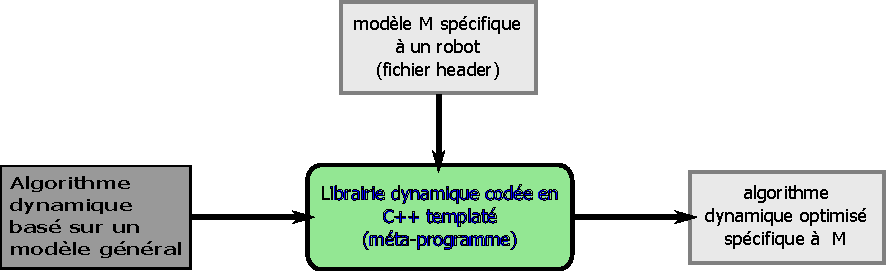
\includegraphics[width=\textwidth]{figs/principeAlgoGenerique.pdf}
\caption{Génération automatique d'algorithmes optimisés et spécialisés}
\end{figure}



\subsection{Le mécanisme de parcours récursif à l'aide de visiteurs} \label{ch_concepts_visiteurs}

On définit, pour le parcours récursif d'un arbre cinématique, deux procédures suivant la méthode d'exploration:
\begin{itemize}
\item[$\centerdot$] \textsc{DepthFirstTraversal} pour un parcours en profondeur d'abord, implémenté sous \emph{métapod} dans la fonction $\mathit{template<visitor, model, node_{id}> \quad struct \quad depth\_first\_traversal()}$
\item[$\centerdot$] \textsc{BackwardTraversal} pour un parcours arrière en remontant l'arbre vers la racine, implémenté sous \emph{metapo} dans la fonction $\mathit{template<visitor, model, node_{id}, end\_node\_{id}> struct backward\_traversal()}$.
 \end{itemize}
\bigskip

\setlength{\columnseprule}{0.5pt}
\begin{multicols}{2}\raggedcolumns\small
    	\begin{spacing}{1.5}
		\begin{pseudocode}[display]{}{}
		\PROCEDURE{DepthFirstTraversal}{visitor,model,i_{start}}
		    \FOREACH i \in \mu(i_{start}) \DO
		        \CALL{DepthFirstTraversalRec}{visitor,model,i_{start}}
		\ENDPROCEDURE \\
		\PROCEDURE{DepthFirstTraversalRec}{visitor,model,i}
        \CALL{visitor.discover}{model,i} \\
        \FOREACH i \in \mu(i) \DO
            \CALL{DepthFirstTraversal}{visitor,model,i} \\
        \CALL{visitor.finish}{model,i}
		\ENDPROCEDURE
	  \end{pseudocode}
	 
		\begin{pseudocode}[display]{}{}
		\PROCEDURE{BackwardTraversalPrev}{visitor,model,i_{start}[,i_{end}]}
		    \COMMENT{$i_{end}$ est optionnel. Par défaut, $i_{end} \GETS 0$.} \\
		    \CALL{BackwardTraversalPrevRec}{visitor,model,\lambda(i_{start}),i_{start},i_{end}}
		\ENDPROCEDURE \\
		\PROCEDURE{BackwardTraversalPrevRec}{visitor,model,i,i_{prev},i_{end}}
		    \COMMENT{$i=\lambda(i_{prev})$.} \\
        \CALL{visitor.discover}{model,i,i_{prev}} \\
        \IF i \neq i_{end}
        \THEN \CALL{BackwardTraversalPrevRec}{visitor,model,\lambda(i),i,i_{end}} \\
        \CALL{visitor.finish}{model,i,i_{prev}}
		\ENDPROCEDURE
	  \end{pseudocode}
	  \end{spacing}
\end{multicols}

\paragraph{Parcours en profondeur et visiteur:}
La procédure \textsc{DepthFirstTraversal} parcours l'arbre cinématique du \emph{model} en profondeur d'abord, par appels récursifs des noeuds enfants, et en partant du noeud $i_{start}$. Chaque noeud visité, sauf le noeud $i_{start}$, est traité par le "visiteur" défini par deux procédures \textsc{visitor.discover} et \textsc{visitor.finish}. Pour chaque noeud visité $i$, \textsc{Discover} définit le traitement à appliquer avant l'exploration des enfants $\mu(i)$. \textsc{Finish} réalise le traitement dans la phase ascendante, \cad après l'exploration de tous les enfants de $i$.

\paragraph{Parcours en arrière:}
La procédure \textsc{BackwardTraversalPrev} parcours l'arbre en partant du noeud $i_start$, et en remontant vers la racine par l'appel récursif du parent du noeud visité, jusqu'au noeud $end\_node$. Comme pour \textsc{DepthFirstTraversal}, pour chaque noeud visité, sauf pour le noeud $i_start$, les fonctions \textsc{visitor.discover} et \textsc{visitor.finish} sont appelées respectivement avant et après l'exploration du noeud parent.

\paragraph{Meta-programmation en template C++:}
La méta-programmation du template C++ nous permet d'obtenir une optimisation extrême de certaines fonctions en invoquant la totalité de leur traitement à la compilation. Ceci requiert une architecture et écriture particulière de la fonction: tous ses paramètres et variables locales sont statiques, des types purs (champ de la classe le plus souvent désigné par $::type$) ou des types dit "wrapper type" (champ le plus souvent désigné par $::value$) représentant des valeurs numériques. Dans le premier cas on est en présence d'une \emph{Métafonction}, dans le deuxième cas en présence d'une \emph{Metafonction numérique} (\cite{bib_metaprogramming} chap.2 section 2.9).


%%%%%%%%%%%%%%%%%%%%%%%%%%%%%%%%%%%%%%%%%%%%%%%%%%%%%%%%%
\chapter{algèbre spatiale selon Roy Featherstone}
%Formalisme compacte et plus adapté :\vspace{0.3cm}
%- au calcul numérique et récursif\vspace{0.3cm}
%- au parcours en profondeur d'abord d'arbres cinématiques\vspace{0.3cm}

\setmyFiguresFile{figures}

L'algorithme de dynamique hybride a été implémenté suivant le formalisme présenté par Featherstone dans son ouvrage \cite{Featherstone} regroupant l'ensemble des algorithmes sur la dynamique des corps rigides: l'algorithme récursif de Newton-Euler (\emph{\gls{acr_rnea}}), l'algorithme "corps rigide composite" (\emph{\gls{acr_crba}}) et l'algorithme de corps articulés (\emph{\gls{acr_aba}}). Ce formalisme est basé sur l'algèbre spatiale, qui définit les grandeurs dynamiques à l'aide d'une notation condensée et efficace, et utilise très souvent des mécanismes récursifs comme le parcours en profondeur de graphes représentant l'arbre cinématique d'un robot. Nous allons présenter dans cette section les fondements de l'algèbre spatiale, ainsi que les algorithmes impliqués dans la construction de l'algorithme hybride: le \gls{acr_rnea} et le \gls{acr_crba}.\\


\section{Algèbre spatiale: définition des vecteurs spatiaux et d'un modèle de système}

L'algèbre spatiale est un système de notation très concis et léger pour décrire la vitesse, l'accélération et les forces appliquées à des corps rigides, à l'aide de vecteurs à six dimensions (tenseurs) dits vecteurs spatiaux. Cette notation réduit grandement la taille des équations de mouvement des modèles cinématique et dynamique du robot. En particulier, elle simplifie la transformation des tenseurs entre les repères liés aux différents corps du robot. Quelques exemples seront donnés après la présentation de ces fondements.\\


\subsection{Vecteurs spatiaux: espaces mathématique et bases}

Pour décrire le mouvement d'un corps rigide dans un espace 3D, et ayant six degrés de liberté, nous devons décrire le déplacement en translation et en rotation. Pour cela, on définit des tenseurs combinant ces deux types de grandeurs dans des espaces de vecteurs à six dimensions (6D). On définit ainsi :\\
\begin{itemize}
\item dans un espace noté $M^{6}$, un tenseur de mouvement pour les vitesses ou accélérations du corps
\item dans l'espace noté $F^{6}$, un tenseur de forces pour les forces et les couples appliqués à ce même corps
\end{itemize}
On définit des bases dans ces espaces, ainsi que les opérateurs : somme, produit scalaire, produit vectoriel.\\
Le vecteur de coordonnée $\underline{m}=[m_{1},...,m_{6}]^T$ représente le vecteur $m$ dans la base ${d_{1},...,d_{6}}$ dans $M^{6}$.
De même, $\underline{f}=[f_{1},...,f_{6}]^T$ représente le vecteur $f$ dans la base ${e_{1},...,e_{6}}$ dans $F^{6}$.
Ces bases sont réciproques, normales :

$$
d_{i}\cdot e_{j}=
\begin{cases}
0 \colon i \neq j\\
1 \colon i = j
\end{cases}
$$

Ainsi le produit scalaire entre ces vecteurs s'exprime:

$$
"\cdot" : M^{6} \times D^{6} \mapsto R
\qquad
\qquad
m \cdot f = \underline{m}^T f
$$

\subsection{Vitesse}\label{ch_algSpa_Vitesse}

On veut exprimer la vitesse d'un corps solide dans l'espace $M^{6}$. On considère un corps en rotation autour d'un axe passant par un point $P$ du solide, avec une vitesse angulaire $w$, et en translation avec une vitesse linéaire $v_{P}$. On défini un repère $R_{O}$ dans l'espace à trois dimensions du solide ($R(O,x,y,z)$).

\dispTwoFig[H]
{1}{Rotation autour d'un point du solide $P$}
{2}{Rotation autour du centre du repère $O$}
{Vitesse d'un objet en mouvement quelconque (translation et rotation simultanées). Un nouveau point de vue pour le vecteur spatial.}
{fig_VitessePointCoincidant}


Soit $P'$ un point quelconque lié au corps solide $C$ (donc fixe dans n'importe quel repère lié au solide). La vitesse du point $P'$ dans $R$ est donnée par	$v_{P'}=v_{P}+\overrightarrow{P'P} \times w$ .\\
On imagine que le solide s'étend maintenant à tout l'espace autour de lui, englobant ainsi le repère $R$. On peut considérer ainsi un champ de vitesses associé au champ de position de tous les points du solide étendu. Soit le point de ce champ coïncidant avec le centre su repère $O$, autrement dit le point lié au solide (étendu) coïncidant avec $O$ au moment où on mesure la vitesse du solide. Soit $v_{O}$ la vitesse du solide en ce point. Il est impératif de remarquer que ce vecteur vitesse n'est pas lié au solide, mais plutôt au point fixe $O$ (voir l'annexe \ref{appx_torseursToalgSpa_torseurs_appl} sur les torseurs). Comme pour le point $P'$ évoqué précedemment, on a:
$$
v_{O} = v_{P} + w \times \overrightarrow{PO}\\
\Leftrightarrow v_{P} = v_{O} - w \times \overrightarrow{PO} = v_{O} + w \times \overrightarrow{OP}
$$

On peut donc voir le corps $C$ comme un solide en translation à la vitesse $v_{O}$ et en rotation autour d'un axe passant par $O$ (parallèle à l'axe défini initialement) à la vitesse angulaire $w$. La vitesse de tout point $P$ de ce solide dans le repère $R(O,x,y,z)$ est alors donnée par:
\begin{equation}
v_{P} = v_{O} + w \times \overrightarrow{OP}
\quad\quad
\footnote{Bien que la vitesse $v_{P}$ soit définie en fonction de $O$, elle ne dépend pas de l'origine choisie puisqu'il s'agit du vecteur vitesse associé à $P$ par le champ de vitesses du solide, qui lui est indépendant de l'origine. En effet, $v_{O}$ et $\overrightarrow{OP}$ dépendent tous deux de $O$, mais ces dépendances se compensent.}
\end{equation}

On veut exprimer les coordonnées de $w$ et $v_{O}$ dans le repère cartésien $R(O,x,y,z)$. Pour cela, on définit la base orthonormée de \emph{Plücker} dans l'espace des tenseurs de mouvement $M^{6}$:\\

\begin{figure}[H]
\minipages[3]{t}{.3}{.3}{.4}
{%
  \dispFig[H]{3}{4cm}{}{}
}{%
  \begin{align*}
  D_{O} = \lbrace &\textbf{d}_{Ox}, \textbf{d}_{Oy}, \textbf{d}_{Oy}, \\
  &\textbf{d}_{x}, \textbf{d}_{y}, \textbf{d}_{z} \rbrace \subset M^{6}
  \end{align*}
}{%
  \begin{tabbing}
  \= $\textbf{d}_{Ox}$ \= vecteur unitaire de rotation autour de $O_{x}$\\
  \> $\textbf{d}_{Oy}$ \> vecteur unitaire de rotation autour de $O_{y}$\\
  \> $\textbf{d}_{Oz}$ \> vecteur unitaire de rotation autour de $O_{z}$\\
  \> $\textbf{d}_{x}$  \> vecteur unitaire de translation le long de $O_{x}$\\
  \> $\textbf{d}_{y}$  \> vecteur unitaire de translation le long de $O_{y}$\\
  \> $\textbf{d}_{z}$  \> vecteur unitaire de translation le long de $O_{z}$\\
  \end{tabbing}
}
\caption{Base de \emph{Plücker} dans $M^{6}$}
\label{fig_basePlucker}
\end{figure}

Voici les coordonnées cartésiennes de $w$ et $v_{O}$, ainsi que leur concaténation constituant les coordonnées du vecteur spatial $\widehat{v}$ dans la base de \emph{Plücker}:\\

\begin{minipage}[c]{.55\textwidth}
$$
\underline{w}=
\begin{bmatrix}
w_{x} \\
w_{y} \\
w_{z}
\end{bmatrix}
\quad \texttt{et} \quad
\underline{v}_{O}=
\begin{bmatrix}
v_{Ox} \\
v_{Oy} \\
v_{Oz}
\end{bmatrix}
\quad \Rightarrow \quad
\underline{\widehat{v}}_{O}=
\begin{bmatrix}
\underline{w} \\
\underline{v}_{O}
\end{bmatrix}
=
\begin{bmatrix}
w_{x} \\
w_{y} \\
w_{z} \\
v_{Ox} \\
v_{Oy} \\
v_{Oz}
\end{bmatrix}
$$
\end{minipage}
\begin{minipage}[c]{.45\textwidth}
\begin{align*}
\quad \texttt{représentant} \quad
\widehat{v} = 
  &w_{x}\textbf{d}_{Ox} + w_{y}\textbf{d}_{Oy} + w_{z}\textbf{d}_{Oz} \\
  &+ v_{Ox}\textbf{d}_{x} + v_{Oy}\textbf{d}_{y} + v_{Oz}\textbf{d}_{z}
\end{align*}
\end{minipage}

\vspace{0.3cm} % retour à la ligne

Le vecteur spatial $\widehat{v}$ rassemble les six composantes représentant complètement les mouvements $\underline{w}$ et $\underline{v}_{O}$ du corps $C$. Ce vecteur a une propriété majeure qui est l'invariance par rapport à la base de \emph{Plücker} choisie. Si on définit deux bases de \emph{Plücker} différentes $D_{O}$ et $D_{P}$, centrées respectivement sur $O$ et $P$, ainsi que les vecteurs spatiaux associés $\widehat{v}$ et $\widehat{v'}$, on obtient:

\begin{align}
\widehat{v}  &= \underline{v}_{O} \cdot D_{O} \notag \\
\widehat{v'} &= \underline{v}_{P} \cdot D_{P} \notag \\
^{D_{O}}\widehat{v} \quad &= \quad ^{D_{O}}\widehat{v'}
\label{equ_invariant}
\end{align}


Les projections de ces deux vecteurs spatiaux $\widehat{v}$ et $\widehat{v'}$ dans la même base de \emph{Plücker} sont identiques \eqref{equ_invariant}. Il faut noter que si les deux bases ont la même orientation, elles auront les mêmes vecteurs unitaires de translation ($\textbf{d}_{x}$, $\textbf{d}_{y}$ et $\textbf{d}_{z}$), mais les vecteurs unitaires de rotations diffèrent si $O \neq P$ ne sont pas confondus, comme illustré dans le l'exemple de cas simple ci-dessous:

\begin{figure}[H]
\begin{center}
  \subfloat[Equivalence des vecteurs de translation.]{\includegraphics[width=.3\textwidth, page=4]{figs/figures}}\hspace{.05\textwidth}
  \subfloat[Visualisation de $\textbf{d}_{Py}$ et $\textbf{d}_{Pz}$ en $O$.]{\includegraphics[width=.3\textwidth, page=5]{figs/figures}}\hspace{.05\textwidth}
  \subfloat[Expression des vecteurs de rotation dans $D_{O}$]
  {%
  \begin{minipage}[t]{.2\textwidth}
  \begin{center}
    \(\begin{aligned}
      \textbf{d}_{Px} &= \textbf{d}_{Ox} \\
      \textbf{d}_{Py} &= \textbf{d}_{Oy}+r \textbf{d}_{z} \\
      \textbf{d}_{Pz} &= \textbf{d}_{Px}-r \textbf{d}_{y}
    \end{aligned}\)
  \end{center}
  \end{minipage}
  }
  \caption{Transformation des vecteurs unitaires de mouvement entre deux bases de \emph{Plücker} de même orientation}  % legende
  \label{fig_transPlucker}    % pour citer le numéro de figure
\end{center}
\end{figure}

Pour rapidement comprendre ces transformations, on peut visualiser un corps tournant autour de l'axe $P_{y}$ à la vitesse $w_{y}$. On définit initialement le vecteur spatial $\widehat{v'}$ en $P$ (\cad considérant l'axe de rotation du corps autour de $P_{y}$) est alors $w_{y}\textbf{d}_{Py}$. Or la vitesse d'un point lié au corps et passant par $O$ (par rapport au repère fixe $R(O,x,y,z)$) vaut $rw_{y}\textbf{d}_{z}$. Le vecteur spatial en $O$ (\cad considérant le corps en rotation autour de l'axe $O_{y}$) est alors $\widehat{v}=\textbf{d}_{Oy}+r\textbf{d}_{z}$.

La propriété d'invariance se vérifie pour tout point $O$ et $P$ fixes dans l'espace et une orientation quelconque des repères $R(O,x,y,z)$ et $R'(P,x,y,z)$. Nous pouvons trouver la démonstration complète de cette propriété d'invariance dans l'annexe \ref{appx_dem}.

\subsubsection*{Composition de vitesses}
On rappelle  la définition de la matrice de sélection $S_k$ d'une articulation $k$ donnée, liant la vitesse spatiale du corps $k$ à la variable articulaire $\dot{q}_k$ (section \ref{ch_algSpa_transformations}). Soit $v_J$ la "vitesse à travers l'articulation $i$", \cad la vitesse du corps $k$ par rapport au corp parent $\lambda(k)$, et soit $\dot{q}_i$ la variable vitesse articulaire associée. On a alors:
\begin{align}
\textnormal{Vitesse du corps $k$ par rapport à $\lambda(k)$ dans le repère $R_k$ lié au corps $k$} : {^kv_J} &= {^kS_k} \: \dot{q}_k \\
\textnormal{Vitesse du corps $k$ par rapport à $\lambda(k)$ dans le repère base $R_0$ lié au corps $0$} : {^0v_J} &= {^0X_k} {^kS_k} \: \dot{q}_k = {^0S_k} \: \dot{q}_k \\
\textnormal{Vitesse du corps $k$ par rapport à $0$ dans le repère $R_0$} : {^0v_k} &= {^0v_{\lambda(k)}} + {^0v_{J}} \\
&= {^0v_{\lambda(k)}} + {^0S_k} \: \dot{q}_k \\
\textnormal{Par récursivité} : v_k &= \sum_{i \in \kappa(k)} {^0S_i} \: \dot{q}_i
\end{align}
Ceci exprime la composition des vitesses des corps supportant le corps $k$.

\paragraph*{Différence entre la notion de vitesse relative à un corps et vitesse exprimée dans le repère dans le repère de \emph{Plücker} de ce même corps:} La différence entre $v_{i:j} = {^0v_{i:j}}$ (vitesse du corps $i$ par rapport à $j$ exprimée en un repère fixe quelconque $R_0$), et $^iv_j = {^iv_{0:j}}$ (vitesse du corps $j$ par rapport à un repère fixe quelconque $R_0$, exprimée dans le repère lié à $i$).
En algèbre spatiale, lorsqu'on note une vitesse spatiale ${^iv_{0:j}}$ exprimée dans le repère lié à un corps $i$ donné, on considère une "photo" instantanée de ce repère, on le considère donc fixe. La composition (somme) des vitesses des différents corps se fait à travers la somme des vecteurs spatiaux, et non pas à travers les matrices de passage $^BX_A$ entre repères de \emph{Plücker}. C'est à dire que si un corps $j$ est immobile par rapport à un autre corps $j$, mais tous les deux sont mobiles par rapport à un repère fixe $R_0$, on a ${^iv_j } = {^iv_{0:j}} \neq 0$.

\subsection{Force}

Nous nous intéressons à présent aux forces appliquées au corps rigide $\emph{C}$. Soit une force $\textbf{f}$ quelconque appliquée au solide. On le définit comme une somme:
\begin{itemize}
\item d'une force linéaire passant par un point donné $P$ de $\emph{C}$
\item d'un couple $\textbf{n}_{P}$ autour d'un axe passant par $P$
\end{itemize}

Comme précédemment, nous considérons le champ de positions du corps $C$ étendu à tout l'espace. nous choisissons un point $O$ fixe dans l'espace. Nous définissons la force 

\subsection{Coordonnées de Plücker et transformation de bases} \label{ch_algSpa_transformations}


\section{construction du modèle du système et de l'équation de mouvement} \label{ch_algSpa_equationMouvement}

\section{Dynamique inverse et \gls{acr_rnea}}

\section{Dynamique directe et \gls{acr_crba}}



\chapter{Implémentation d'un algorithme dynamique hybride pour la prise en compte des liaisons flexibles}

L'algorithme Dynamique Hybride est une généralisation de la dynamique directe et de la dynamique indirecte (\gls{acr_rnea}). En effet, il applique la dynamique directe aux articulations dont on connaît les couples ou forces appliquées, et la dynamique inverse aux articulations dont on connaît les accélérations. Toutes les inconnues sont ainsi résolues.\\
Cet algorithme est décomposé en cinq étapes incluant le déroulement complet d'un \gls{acr_rnea}, ainsi que d'un \gls{acr_crba} pour la construction de la matrice d'inertie du système entier. Ces deux algorithmes sont utilisés sous une forme adaptée à l'algorithme hybride, et j'ai dû apporter certains compléments afin de permettre leur intégration dans l'algorithme principal.\\
Dans les sections précédentes, nous avons posé les bases de l'algèbre spatiale des torseurs cinématiques et dynamiques, ainsi que la modélisation généralisée d'un arbre cinématique (\emph{modèle de sytème} du robot). Nous allons décrire dans cette section la définition de l'\emph{algorithme hybride}, et son implémentation qui s'est déroulée sur plusieurs phases:\\
\begin{itemize}
  \item[$\centerdot$] Analyse de l'algorithme tel qu'il est présenté par Featherstone (\cite{bib_featherstone} chap.9). Lors de cette phase, j'ai dû apporter certains compléments au calcul des éléments de la matrice d'inertie, face à la proposition initiale de Featherstone non totalement explicitée, afin de permettre le calcul de toutes les inconnues.
  \item[$\centerdot$] Analyse des dépendances:
  \begin{itemize}
    \item[-] méthodes (\gls{gls_jcalc}, méthodes de résolution des systèmes linéaires)
    \item[-] algorithmes (\gls{acr_rnea} et \gls{acr_crba}) réutilisés par l'\emph{hybride dynamics}
    \item[-] impacts sur la définition du modèle du système dynamique (modèle \gls{acr_urdf}) et sur le parseur de modèle URDF pour la prise en compte des spécificités de l'algorithme hybride
  \end{itemize}
  \item[$\centerdot$] Identification des algorithmes déjà implémentés, à modifier ou à implémenter entièrement dans la librairie dynamique \gls{gls_metapod}
  \item[$\centerdot$] Identification et prise en main des outils logiciels pour la manipulation de matrices et systèmes linéaires (matrices et solveurs \gls{gls_eigen} \cite{bib_eigen})
  \item[$\centerdot$] Implémentation d'une version modifiée des algorithmes \gls{acr_rnea} et \gls{acr_crba} adaptée à l'\emph{hybrid dynamics}, ainsi que de l'algorithme principal dans \emph{metapod}
  \item[$\centerdot$] Optimisation logique visant à réduire le nombre d'étapes de calcul, ainsi que l'optimisation de la compilation et exécution de ces étapes à l'aide des thecniques de \emph{Meta-programmation}
\end{itemize}


\section{l'algorithme hybride en quatre étapes}

\subsection{mise en place de l'équation de mouvement et séparation des variable connues/inconnues}

Nous considérons l'équation de mouvement relative à un arbre cinématique générique (à base fixe ou flottante), sous la forme matricielle (\cite{bib_featherstone} chap.6) comme suit:

\begin{equation} \label{equ_equationMvt}
H(q)\ddot{q} + C(q,\dot{q},f^x) = \tau
\end{equation}

\medskip

\begin{wrapfigure}{r}{0.5\textwidth}
  \begin{flushright}
  \begin{minipage}[t]{0.45\textwidth}
  \begin{description}
    \item[$q, \dot{q}, \ddot{q}$ :] vecteurs de position, vitesse, accélération
    \item[$\tau$ :] forces/couples moteurs (internes)
    \item[$H$ :] matrice des termes inertiels
    \item[$C$ :] forces de précontrainte extérieures
  \end{description}
  \end{minipage}
  \end{flushright}
\end{wrapfigure}

qui regroupe les éléments dynamiques décrits ci-contre: vecteurs de position / vitesse / accélération des articulations; les couples moteurs (internes) appliqués aux articulations; les forces extérieures au système éventuelles appliquées aux corps et ramenés aux articulations; la matrice inertielle dans l'espace de configuration et le vecteur de forces de précontrainte ou "bias" (force de Coriolis, la pesanteur, etc).
Pour simplifier les notations, les dépendances $q$, $\dot{q}$ et $f^x$ des coefficients $H$ et $C$ de l'équation seront omises. Les variables sont les forces/couples $\tau$ et les accélérations $\ddot{q}$.\\
Pour chaque articulation $i$, on connaît soit le couple appliqué soit l'accélération. L'objectif est de calculer toutes les variables inconnues. Cela passe par une mise en forme de l'équation de mouvement, visant à ramener toutes les variables inconnues du même côté de l'égalité, et laisser toutes les variables connues de l'autre côté.

\subsubsection{Permutation des vecteurs de variables et de coefficients}

\setmyFiguresFile{hybridDynamics4etapes}

\begin{wrapfigure}{r}{0.5\textwidth}
  \begin{center}
    \incFig[1]{.3\textwidth}
    \caption{Graphe de l'arbre cinétique}
    \label{fig_chdaArbreK1}
  \end{center}
\end{wrapfigure}

Soit le sous-ensemble d'articulations pour lesquelles on connaît le couple $\tau$ de forces appliquées. On désigne cet ensemble celui des articulations en mode "forward-dynamics" ou "articulations \emph{fd}" ou encore \emph{fd}. L'ensemble complémentaire regroupe les "articulations en mode "inverse-dynamics" ou "id". l'ensemble \emph{fd} est supposé connu et fournit par le modèle du système. Nous noterons $n_{\emph{fd}}=\vert fd \vert$, $n_{\emph{id}}=\vert id \vert$ et $n_{dof}=n_{\emph{fd}}+n_{\emph{id}}=\vert \ddot{q} \vert$. Il s'agit là d'un impact sur la définition du modèle standard \gls{acr_urdf} et du "parseur" respectif, tous deux définis à la base dans le standard \gls{acr_ros}.\\
Avant de pouvoir déplacer toutes les variables inconnues du même côté de l'égalité, nous devons les regrouper. Pour cela, nous appliquons une permutation à tous les éléments de l'équation de mouvement. Commençons par les vecteurs de variables et de coefficients. Nous définissons ainsi la matrice de permutation $\mathbf{Q}$ qui réordonne les vecteurs $q$, $\dot{q}$, $\ddot{q}$ en plaçant les variables inconnues en premier. Considérons l'exemple simple ci-contre. Comme vu dans l'établissement de l'équation de mouvement au chapitre \ref{ch_algSpa_equationMouvement}, l'ordre des variables $q_i$, $\dot{q}_i$, $\ddot{q}_i$, dans les vecteurs respectifs, est donné suivant le parcours de l'arbre cinétique en profondeur d'abord:

\begin{Parallel}[v]{.4\textwidth}{.5\textwidth}
\ParallelLText{%
\begin{align*}
\ddot{q} &= 
\begin{bmatrix}
  \ddot{q}_1 & \ddot{q}_2 & \textcolor{blue}{\ddot{q}_4} & \ddot{q}_5 & \textcolor{blue}{\ddot{q}_3} & \ddot{q}_6 & \ddot{q}_7
\end{bmatrix}^T \\
\medskip
Q &= 
\begin{bmatrix}
  0 & 0 & 1 & 0 & 0 & 0 & 0 \\
  0 & 0 & 0 & 0 & 1 & 0 & 0 \\
  1 & 0 & 0 & 0 & 0 & 0 & 0 \\
  0 & 1 & 0 & 0 & 0 & 0 & 0 \\
  0 & 0 & 0 & 1 & 0 & 0 & 0 \\
  0 & 0 & 0 & 0 & 0 & 1 & 0 \\
  0 & 0 & 0 & 0 & 0 & 0 & 1  
\end{bmatrix}
\end{align*}
}
\ParallelRText{%
\begin{align*}
n_{dof}&=7, n_{\emph{fd}}=2, n_{\emph{id}}=5 \\
Q \ddot{q} &= 
\begin{bmatrix}
  \textcolor{blue}{\ddot{q}_4} & \textcolor{blue}{\ddot{q}_3} & \ddot{q}_1 & \ddot{q}_2 & \ddot{q}_5 & \ddot{q}_6 & \ddot{q}_7
\end{bmatrix}
=
\begin{bmatrix}
  \underline{\ddot{q}_1} \\
  \underline{\ddot{q}_2}
\end{bmatrix} \\
\textnormal{ et de même } \\
Q \tau &= 
\begin{bmatrix}
  \underline{\tau_1} \\
  \underline{\tau_2}
\end{bmatrix}
\qquad \textnormal{et} \qquad
Q C = 
\begin{bmatrix}
  C_1 \\
  C_2
\end{bmatrix}
\end{align*}
}
\end{Parallel}
\medskip
Avec $\underline{\ddot{q}_1}$ et $\underline{\tau_1}$ les sous-vecteurs des variables (\emph{fd}), de dimensions $(n_{\emph{fd}} \times 1)$, et $\underline{\ddot{q}_2}$ et $\underline{\tau_2}$ les sous-vecteurs des variables (\emph{id}), de dimensions $(n_{\emph{id}} \times 1)$. Pour alléger la notation, on notera ces vecteurs tout simplement $\ddot{q}_1$, $\ddot{q}_2$, $\tau_1$ et $\tau_2$.

\subsubsection{Quelques propriétés de $Q$}

\begin{flushleft}
\begin{itemize}
\item[•] Il y a un seul élément à 1 par ligne et un seul élément à 1 par colonne, tous les autres éléments étant à 0
\item[•] D'après la forme de $Q$, on montre facilement que pour toute matrice carrée $m$, le produit à gauche $m'=Qm$ permute les lignes de $m$, et le produit à droite $m'=mQ$ permute les colonnes. En effet, dans le produit $m'=Qm$, chaque élément $Q_{ij}$ à 1 affecte la ligne $j$ de $m$ à la ligne $i$ de $m'$. Pour la permutation de colonnes, il suffit de passer par la transposée de $m$. Soit $Q'$ la transformation permutant les colonnes:

\begin{center}
\(
\begin{aligned}
&Q : m \mapsto Q m \qquad \textnormal{est une permutation de lignes.} \\
&\textnormal{... on transpose les matrices en relation. Les lignes deviennent des colonnes,} \\
&\textnormal{qui héritent donc du même ordonnancement ...} \\
&Q': m^T \mapsto (Q m)^T = m^T Q^T \quad \implies Q'=Q^T \\
&Q^T: m \mapsto m Q^T \qquad \textnormal{est donc une permutation de colonnes.} \\
\end{aligned}
\)
\end{center}
\medskip
\item[•] Toute matrice de permutation est inversible et $Q^{-1}=Q^T$. Cette propriété se démontre simplement grâce aux propriétés de la transposition de matrice. Soit une matrice quelconque $A$. $(AA^T)^T=(A^T)^TA^T=AA^T$, donc la matrice $AA^T$ est une matrice symétrique. On en déduit que $QQ^T$ est une matrice symétrique. Or $Q^T$, ainsi que $Q(Q^T)$ (permutation des lignes de $Q^T$), ont les mêmes propriétés que $Q$ (un seul élément à 1 par ligne). On en déduit que $QQ^T$ est une matrice symétrique avec un seul élément à 1 par ligne, ce qui correspond à la matrice identité $I$.
\end{itemize}
\end{flushleft}

Ces propriétés sont décrites plus en détail en annexe \ref{appx_algLineaire}.

\subsubsection{permutation de la matrice d'inertie et reformulation de l'équation de mouvement}

On applique la permutation $Q$ à tous les éléments de l'équation de mouvement \eqref{equ_equationMvt}:
\begin{spacing}{1.5}
\begin{align}
&H \ddot{q} + C = \tau \notag \\
\iff &H \ddot{q} = \tau - C \notag \\
\iff &Q H \ddot{q} = Q \tau - Q C \label{equ_local_eqMvt_1} \\
\textnormal{or} \qquad &Q^T Q = I \iff \ddot{q} = Q^T Q \ddot{q} \qquad \textnormal{donc} \notag \\
\eqref{equ_local_eqMvt_1} \iff &(Q H Q^T) (Q \ddot{q}) = Q \tau - Q C \notag \\
\iff 
&\begin{bmatrix}
  H_{11} & H_{12} \\
  H_{21} & H_{22}
\end{bmatrix} 
\cdot
\begin{bmatrix}
  \ddot{q}_{1} \\
  \ddot{q}_{2}
\end{bmatrix} 
= 
\begin{bmatrix}
  \tau_{1} \\
  \tau_{2}
\end{bmatrix} 
-
\begin{bmatrix}
  C_{1} \\
  C_{2}
\end{bmatrix} \label{equ_local_eqMvt_2}
\end{align}
\end{spacing}

où $H_{11}$ est de dimensions ($n_{fd} \times n_{fd}$), $H_{12}$ de dimensions ($n_{fd} \times n_{id}$), $H_{21}$ est de dimensions ($n_{id} \times n_{fd}$) et $H_{22}$ de dimensions ($n_{id} \times n_{id}$).
\subsubsection{regroupement des inconnues à gauche de l'équation}

Il ne reste plus qu'à regrouper $\ddot{q}_1$ et $\tau_2$ à gauche de l'équation:

\begin{alignat}{2}
\eqref{equ_local_eqMvt_2} \iff
&\begin{bmatrix}
  H_{11} \\
  H_{21}
\end{bmatrix} 
\cdot \ddot{q}_1
+
\begin{bmatrix}
  H_{12} \\
  H_{22}
\end{bmatrix}
\cdot \ddot{q}_2
&&=
\begin{bmatrix}
  \tau_1 \\
  0
\end{bmatrix} 
+
\begin{bmatrix}
  0 \\
  I
\end{bmatrix} 
\cdot \tau_2
-
\begin{bmatrix}
  C_{1} \\
  C_{2}
\end{bmatrix} \notag \\
\notag \\
\iff
&\begin{bmatrix}
  H_{11} \\
  H_{21}
\end{bmatrix} 
\cdot \ddot{q}_1
+
\begin{bmatrix}
  0 \\
  -I
\end{bmatrix} 
\cdot \tau_2
&&=
\begin{bmatrix}
  \tau_1 \\
  0
\end{bmatrix} 
-
\begin{bmatrix}
  H_{12} \\
  H_{22}
\end{bmatrix}
\cdot \ddot{q}_2
-
\begin{bmatrix}
  C_{1} \\
  C_{2}
\end{bmatrix} \label{equ_equationMvt_dynHyb1} \\
\notag \\
\iff
&\begin{bmatrix}
  H_{11} & 0 \\
  H_{21} &  -I
\end{bmatrix} 
\cdot
\begin{bmatrix}
  \ddot{q}_1 \\
  \tau_2
\end{bmatrix} 
&&=
\begin{bmatrix}
  \tau_1 \\
  0
\end{bmatrix} 
-
\begin{bmatrix}
  C'_{1} \\
  C'_{2}
\end{bmatrix} \label{equ_equationMvt_dynHyb2}
\end{alignat}
\begin{align}
&\textnormal{Avec} \qquad
\begin{bmatrix}
  C'_{1} \\
  C'_{2}
\end{bmatrix}
=
\begin{bmatrix}
  C_{1} \\
  C_{2}
\end{bmatrix}
+
\begin{bmatrix}
  H_{12} \ddot{q}_2 \\
  H_{22} \ddot{q}_2
\end{bmatrix} \label{equ_cPrime}
\end{align}
\\
Nous avons ainsi obtenu l'équation de mouvement pour la dynamique hybride.

\subsubsection{implémentation}

Voici un schéma fonctionnel de du parseur URDF.

%include figure

\begin{itemize}
  \item[représentation de la classification \emph{fd} / \emph{id}] Définition d'un attribut désignant le type d'articulation \emph{fd} ou \emph{id} dans le modèle \gls{acr_urdf} source et dans le modèle du système dérivé dans l'environnement de \emph{metapod} (fichier "header" destinataire).
  \item[interprétation du modèle URDF dans \emph{metapod}] Reverse engineering du parseur URDF et implémentation Méthode de conversion ("parsing") de la source à la destination pour extraire ces attributs de classification.
\end{itemize}
\bigskip
La résolution de l'équation de mouvement de la dynamique hybride se fait en quatre étapes, données dans l'algorithme de dynamique hybride (\cite{bib_featherstone} section 9.1 p.173), et que nous décrivons dans les sections suivantes:
\begin{enumerate}
\item calculer $C'$ d'après l'équation \eqref{equ_equationMvt_dynHyb2}
\item calculer $H_{11}$
\item résoudre $H_{11} \ddot{q}_1 = \tau_1 - C'_1$
\item calculer $\tau_2$ d'après l'équation \eqref{equ_equationMvt_dynHyb2}
\end{enumerate}


\subsection{calcul de C'}
%description de l'algorithme RNEA modifié

$C'$ est l'ensemble des forces et couples de forces motrices $\tau$ assurant une accélération nulle pour les articulations \emph{fd} ($\ddot{q}_1=0$) et l'accélération donnée $\ddot{q}_2$ pour les articulations \emph{id}. en effet on obtient:

\begin{equation}
\textnormal{Pour} \quad \ddot{q}=
\begin{bmatrix}
  0 \\
  \ddot{q}_2
\end{bmatrix}
: \quad
\eqref{equ_equationMvt_dynHyb2} \iff
\begin{bmatrix}
  0 \\
  -I
\end{bmatrix} 
\cdot \tau_2
=
\begin{bmatrix}
  \tau_1 \\
  0
\end{bmatrix} 
-
\begin{bmatrix}
  C'_1 \\
  C'_2
\end{bmatrix}
\iff
\begin{bmatrix}
  C'_1 \\
  C'_2
\end{bmatrix}
=
\begin{bmatrix}
  \tau_1 \\
  \tau_2
\end{bmatrix} 
\end{equation}
\medskip
Les composantes $C'_1$ et $C'_2$ s'obtiennent donc en calculant les couples moteurs $\tau_1$ et $\tau_2$\footnote{%
Dans l'équation \eqref{equ_equationMvt_dynHyb1}, les matrices ou vecteurs $H_{11}$, $H_{21}$, $H_{22}$, $C_1$ et $C_2$ sont constants par rapport aux variables $\ddot{q}$ et $\tau$. Sous l'hypothèse \(\ddot{q}=\begin{bmatrix} 0 & \ddot{q}_2\end{bmatrix}^T\), la valeur de $C'$ est directement fixée par la relation \eqref{equ_cPrime}, et reste valable pour la suite de la résolution du problème. Par contre, $\tau_1$ et $\tau_2$ sont des variables déterminées par la fonction $ID$, et valables uniquement sous l'hypothèse \(\ddot{q}=\begin{bmatrix} 0 & \ddot{q}_2\end{bmatrix}^T\). Leurs valeurs intermédiaires servent uniquement à calculer $C'$.%
} grâce à la fonction de dynamique inverse (\gls{gls_rnea}) suivante:

\begin{equation}
C'=ID \left( q,\dot{q},Q^T
\begin{bmatrix}
  0 \\
  \ddot{q}_2
\end{bmatrix} \right)
\end{equation}

Parmi les paramètres classiques de la fonction $ID$, nous avons remplacé $\ddot{q}$ par 
\(Q^T \begin{bmatrix} 0 & \ddot{q}_2 \end{bmatrix}^T\), 
ce qui correspond à mettre à 0, dans le vecteur original $\ddot{q}$, toutes les variables qui étaient regroupées dans le vecteur réordonné $\ddot{q}_1$.\\


\subsubsection{implémentation}

\begin{itemize}
  \item[•] choix de la méthode de permutation de la librairie Eigen: construction d'un objet "permutation de matrices" à partir des classes Eigen (vecteur de permutation \emph{PermutationBase} incluant des méthodes optimisées de permutation de lignes et colonnes, forme matricielle \emph{PermutationMatrix} pour la multiplication directe $Qm$ ou $mQ^T$.)
  \item[•] remplissage du vecteur de permutation: Choix de l'emplacement du calcul de ce vecteur dans l'une des phases successives:
  \begin{itemize}
    \item de génération du fichier de modèle du système dans l'architecture \emph{metapod}
    \item phase de compilation du fichier de modèle et de \emph{metapod}
    \item exécution de l'algorithme de dynamique hybride
  \end{itemize}
\end{itemize}
\medskip
Nous pouvons visualiser ci-dessous les opérations exécutées sur le vecteur d'entrée $\ddot{q}$ pour obtenir la forme désirée \(Q^T \begin{bmatrix} 0 & \ddot{q}_2 \end{bmatrix}^T\):
\begin{equation*}
\ddot{q} \xmapsto[\textnormal{permutation $Q$}]{} 
\begin{bmatrix}
  \ddot{q}_1 \\
  \ddot{q}_2
\end{bmatrix}
\xmapsto[\textnormal{mettre les $n_{\emph{fd}}$ premiers termes à 0}]{} 
\begin{bmatrix}
  0 \\
  \ddot{q}_2
\end{bmatrix}
\xmapsto[\textnormal{permutation inverse $Q^T$}]{} 
\left. \ddot{q} \right\vert_{\ddot{q}_1=0} = Q^T
\begin{bmatrix}
  0 \\
  \ddot{q}_2
\end{bmatrix}
\end{equation*}
\medskip
Et ci-dessous le calcul de $C'_1$ et $C'_2$:
\begin{equation*}
\left. \ddot{q} \right\vert_{\ddot{q}_1=0} \xmapsto[C'=ID(q,\dot{q},\left. \ddot{q} \right\vert_{\ddot{q}_1=0})]{} C'
\xmapsto[\textnormal{permutation $Q$}]{} 
\begin{bmatrix}
  C'_1 \\
  C'_2
\end{bmatrix}
\end{equation*}


\subsection{calcul de H11 (sous-matrice d'inertie)}
%description de la construction de H et optimisation par défaut "branch sparsity"

Il faut à présent construire la sous-matrice d'inertie $H_{11}$. Plusieurs méthodes sont proposées dans l'algèbre spatiale selon Featherstone (\cite{bib_featherstone} section 9.1) . La plus simple, moins performante, consiste à:
\begin{itemize}
\item[•] calculer la matrice $H$ complète
\item[•] la réordonner suivant la permutation $Q$: $H'=Q H Q^T$
\item[•] Et finalement extraire la sous-matrice $H_{11}$ = $(h_{ij})_{1 \leqslant i \leqslant n_{fd},1 \leqslant j \leqslant n_{fd}}$
\end{itemize}
\bigskip
La deuxième méthode, beaucoup plus performante dans le cas où $n_{\emph{fd}}$ est signicativement plus petit que $n_{dof}$, consiste à modifier l'algorithme \gls{acr_crba}, de sorte à le réduire aux seuls calculs produisant les termes de $H_{11}$. Cette méthode sera abordée en détail dans la section sur les optimisations \ref{ch_impl_optimisation}.

Nous avons choisi la première solution pour une première implémentation, dans le but de répartir la complexité de la tâche à entreprendre, et de se focaliser sur la validation des résultats numériques ainsi que de leurs précision.\\
\textbf{Remarque:} le \gls{acr_crba} original inclut déjà une première optimisation qui consiste à exploiter la sparsité de la matrice $H$, \cad à ne pas recalculer les termes nuls ($\forall q$) de $H$ induits par la topologie de l'arbre cinématique du robot. Plus précisément, cette sparsité est dûe à la nature des liaisons entre les corps du robot. Typiquement, pour deux corps $c_i$ et $c_j$ du système n'ayant aucun lien \emph{parent} - \emph{enfant} (voir chap. \ref{ch_algSpa_equationMouvement}), les coefficients respectifs dans la matrice d'inertie, $H_{ij}$ et $H_{ji}$, sont nuls.

\subsubsection{Implementation}

Cette étape ne présente aucune difficulté particulière. Nous enchaînons les opérations suivantes pour générer la matrice $H_{11}$:

\begin{equation*}
q \xmapsto[CRBA(modèle,q)]{} 
H 
\xmapsto[\textnormal{permutation $Q$ de matrice carrée}]{} 
Q H Q^T = 
\begin{bmatrix}
  H_{11} & H_{12} \\
  H_{21} & H_{22}
\end{bmatrix}
\xmapsto[\textnormal{extraire la matrice $H_{11}$ de $H$}]{} H_{11}
\end{equation*}

COMPLETER: décrire les fonctions Eigen et outils metapod utilisés


\subsection{résolution du système linéaire}
%=> Eigen solver, ddq1

La relation matricielle \eqref{   equ_equationMvt_dynHyb2} se décline en deux équations. La première nous permet de calculer ici $\ddot{q}_1$, et la deuxième nous permettra de calculer $\tau_2$ dans l'étape 5 de l'algorithme global. Calculons $\ddot{q}_1$:

\begin{equation}
H_{11} \ddot{q}_1 = \tau_1 - C'_1 \\
\iff \ddot{q}_1 = H_{11}^{-1} (\tau_1 - C'_1)
\end{equation}

Si $H_{11}$ est inversible. Justement, il est important de noter ici que \textbf{$H$ et $H_{11}$ sont définies positives et symétriques}, et toute matrice définie positive est inversible \cite{bib_matriceDefiniePositive_1} \cite{bib_matriceDefiniePositive_2}. On connaît ces propriétés à la base pour $H$. Intéressons-nous alors aux propriétés de $H_{11}$ qui en découlent:
\begin{flushleft}
\begin{itemize}
\item[•] Symétrique:
\begin{equation*}
\textnormal{H est symétrique}  \iff   H = H^T \iff (Q H Q^T)^T = Q (Q H)^T = Q (H^T Q^T) = Q H Q^T
\end{equation*}
Donc la matrice permutée $Q H Q^T$ est également symétrique.\medskip
\item[•] Définie positive: une matrice réelle M carrée de dimension $n \times n$ est définie positive si $x^T H x > 0$ pour tout vecteur colonne $x$, réel et non nul \cite{bib_matriceDefiniePositive_2}:
\begin{align*}
\textnormal{H définie positive} \iff  &\forall x: x^T H x > 0 \\
\textnormal{or} \quad &x^T (Q H Q^T) x = (x^T Q) H ((Q^T x)^T)^T = (x^T Q) H (x^T Q)^T = y H y^T > 0 \quad \forall y \\
\implies &x^T (Q H Q^T) x > 0 \\
\textnormal{où} \quad &y = x^T Q \quad \textnormal{est un vecteur colonne réel quelconque.}
\end{align*}
Donc la matrice permutée $Q H Q^T$ est également définie positive.\medskip
\item[•] Par construction, la matrice carrée $H_{11}$ hérite de ces propriétés.
\end{itemize}
\end{flushleft}
\medskip
Ainsi, le calcul de $\ddot{q}_1$ peut passer par l'inversion directe de $H_{11}$ pour des systèmes de petite taille (quelques degrés de libertés). Mais pour des systèmes de grande taille, comme par exemple un robot humanoïde à 35 degrés de liberté,  il faudra résoudre le système linéaire définit comme suit:

\begin{align}
&A x = b \notag \\
&\textnormal{Avec:   $A = H_{11}$ ,  $b = \tau_1 - C'_1$  et  $x=\ddot{q}_1$}
\end{align}

Pour résoudre ce système d'équations linéaires, il faudra utiliser une méthode dite de décomposition de la matrice $A$. Il existe de nombreuses méthodes de décomposition en analyse numérique, souvent aussi appelées factorisations, dont le choix dépend d'une série de critères comme:
\begin{itemize}
\item[•] les conditions sur la nature de la matrice $A$ (carrée, inversible, définie positive, semi-définie positive, définie négative)
\item[•] un compromis entre la performance d'exécution, la précision et la stabilité ou robustesse. La robustesse mesure la fiabilité des résultats et à quel point la précision de ces résultats peut diverger en fonction des valeurs de la matrice $A$. Certaines décompositions nécessitent un pré-conditionnement de cette matrice qui peut changer sa nature (permutation de lignes, factorisation, etc)
\item[•] opérations supplémentaires sur la matrice $A$ en plus de la résolution du système linéaire
\item[•] des optimisations intrinsèques à l'algorithme comme le traitement de la matrice par blocs
\item[•] l'exploitation de la parallélisation dans les processeurs multi-cœur via l'OpenMP (\gls{gls_openMP} \cite{bib_openMpWikipedia} \cite{bib_openMPspecs}). Parallélisation implicite: l'algorithme exploite certaines routines parallélisées des processeurs (ex: produits de matrices). Parallélisation explicite: l'algorithme lui-même est parallélisé
\item[•] la disponibilité de l'algorithme dans les librairies de calcul qui seront utilisées dans ce projet (Eigen, Lapack).
\end{itemize}
\medskip
Une description un peu plus détaillée de ces algorithmes sera donnée par  la suite.

\subsubsection{Implémentation}

\`{A} ce stade, les coefficients $A$ et $b$ du système d'équations linéaire $Ax=b$ sont connus. Il faut à présent choisir l'\textbf{algorithme de décomposition approprié} pour le résoudre. L'ensemble des composants logiciels liés à la plateforme robotique de \textbf{HRP2} utilisent majoritairement la librairie dynamique d'outils matriciels \emph{Eigen}. Parmi ces composant on distingue:
\begin{itemize}
\item la librairie \emph{metapod} d'algorithmes de dynamique directe et inverse
\item la \emph{\gls{acr_sot}}, intégrée dans \textbf{HRP2}
\item les composants dédiés à la génération de mouvements et à la simulation (\emph{HPP})
\end{itemize}

En accord avec l'état de ces composants, et avec la stratégie de leur développement et maintenance menée par l'équipe \emph{Gepetto}, l'emploi des méthodes d'\emph{Eigen} était prioritaire dans la mesure de leur disponibilité et compatibilité avec la nature des algorithmes clients. J'ai dressé dans un premier temps la liste complète des algorithmes de décomposition fournis dans \emph{Eigen}, suivant les critères mentionnés plus haut. En voici la description résumée:

\begin{description}
\item[La décomposition $LU$:] il s"agit d'une méthode de décomposition d'une matrice comme produit d'une matrice triangulaire inférieure $L$ (comme "lower", inférieure) et une matrice triangulaire supérieure $U$ (comme "upper", supérieure): $A=LU$ \cite{bib_decompositionLUwikipedia} \cite{bib_decompositionLU_2}
\item[La décomposition Pivot $LU$ ou $PivLU$] dans les cas où $A$ n'admet pas de décomposition $LU$, sauf si on applique une certaine permutation aux lignes de $A$. On obtient alors la forme: $A=PLU$, où $P$ est une matrice de permutation. Cette décomposition a deux versions, la partielle et la complète. La version complète a une approche générique, et entre autres, calcule le rang de la matrice $A$ et vérifie si celle-ci est inversible. La version partielle n'effectue pas cette vérification, et minimise les calculs nécessaires pour atteindre le résultat final. La version partielle est donc plus rapide, mais plus sensible aux erreurs d'arrondi \cite{bib_decompositionLU_1} section 1.3.1, pages 25-26.
\item[•]
\end{description}

Et un tableau regroupant les caractéristiques et contraintes spécifiques à chacun de ces algorithmes \cite{bib_eigen_tutorial_catalogue}:

\begin{figure}[H]
\centering
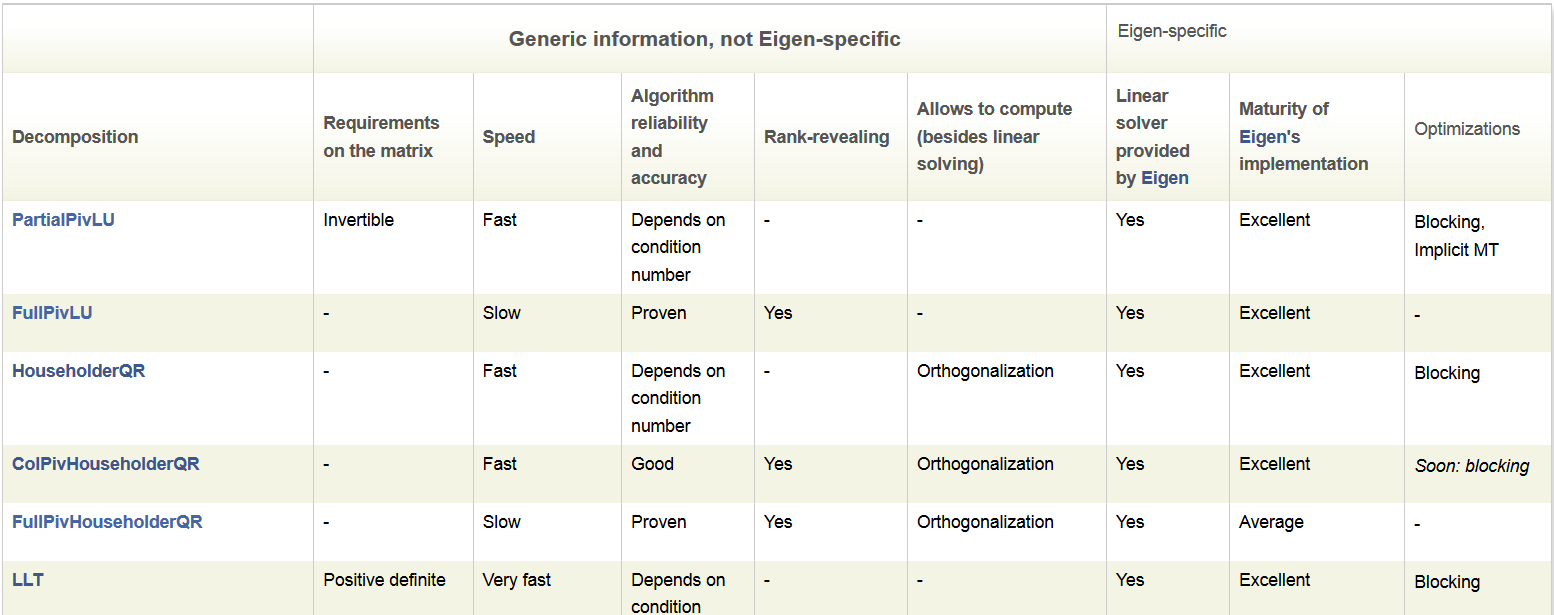
\includegraphics[width=\textwidth]{figs/decompositionCatalogueEigen1.png}
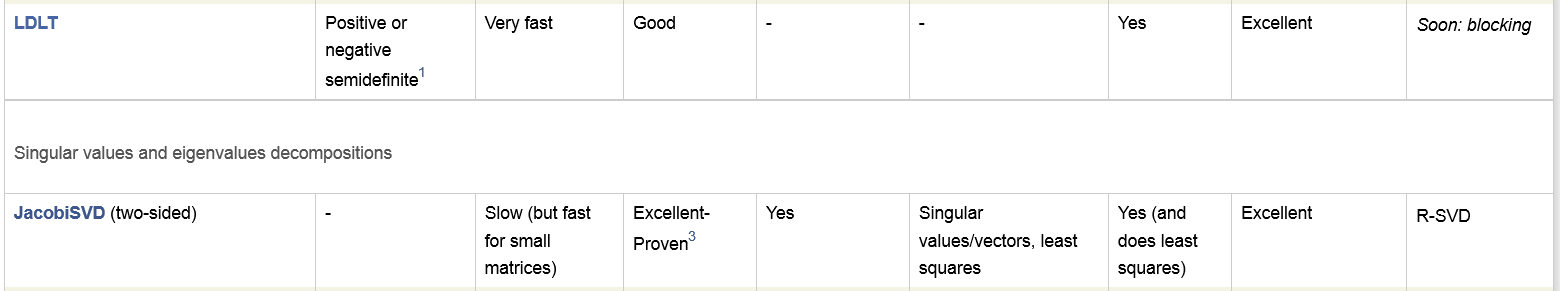
\includegraphics[width=\textwidth]{figs/decompositionCatalogueEigen2.png}
\end{figure}

Tous ces algorithmes ont atteint une très bonne maturité d'implémentation dans la librairie \emph{Eigen}, à part FullPivHouseholderQR, qui est pourtant le plus robuste mais aussi plus lent. Parmi les plus rapides, on trouve les algorithmes de Cholesky, le LLT et le LDLT. Ils intègrent l'optimisation du traitement par blocs et bénéficient quand même d'une bonne fiabilité et précision. Leurs performances bénéficient des conditions les plus restrictives sur la matrice $A$:
\begin{itemize}
\item[\textbf{• LLT:}] $A$ doit être définie positive et symétrique
\item[\textbf{• LDLT:}] $A$ doit être semi-définie positive ou négative
\end{itemize}

%VERIFIER: Comment montrer que H est définie positive
Nous choisissons dans un premier temps l'algorithme le plus restrictif, \emph{LLT}, puisque comme vu précédemment, $H$ et $H_{11}$ sont définies positives. Cette décomposition est particulièrement efficace dans le cas de problèmes symétriques de la forme: $D^* D x = b$ \cite{bib_eigen_LLT_desc} où $D$ est une matrice diagonale. Le problème posé ici ne vérifie pas cette condition.
%VERIFIER: vérifier avec Olivier.
De plus, la décomposition \emph{LLT} devient instable si la matrice est semi-définie positive, or l'algorithme n'intègre pas la vérification de cette condition. Aussi, le calcul des termes de la matrice triangulaire $L$ utilise la division par des racines carrées, ce qui est une source potentielle d'instabilité. La décomposition \emph{LDLT} est plus robuste, évitant l'emploi de racines carrées, comme on peut voir dans comparaison des deux algorithmes ci-dessous:

COMPLETER: comparer les complexités O()


Il faut tester les deux algorithmes sur notre système linéaire et vérifier dans chaque cas la stabilité et précision des résultats, ainsi que la vitesse d'exécution.

voici les étapes réalisées pour la résolution du système linéaire:

COMPLETER: fonctions Eigen et outils metapod utilisés

Il ne nous reste plus que le calcul du vecteur $\tau_2$.


\subsection{résolution de tau2 et reconstruction des vecteurs de sortie ddq et tau}

Nous reprenons maintenant la deuxième équation du système linéaire \eqref{equ_equationMvt_dynHyb2}:
\begin{spacing}{1.5}
\begin{align}
&H_{21} \ddot{q}_1 - \tau_2 = -C'_2 \notag \\
\iff
&\tau_2 = C'_2 + H_{21} \ddot{q}_1 \label{equ_tau}
\end{align}
\end{spacing}

Cette équation représente la deuxième ligne de la relation matricielle proposée par Featherstone \cite{bib_featherstone} section 9.1 page 173:

\begin{align}
\eqref{equ_equationMvt_dynHyb1}
&\iff
\begin{bmatrix}
\tau_1 \\ 
\tau_2
\end{bmatrix} 
=
\begin{bmatrix}
C'_1 \\ 
C'_2
\end{bmatrix} 
+
\begin{bmatrix}
H_{11} \ddot{q}_1 \\ 
H_{21} \ddot{q}_1
\end{bmatrix} \iff
Q^T
\begin{bmatrix}
\tau_1 \\ 
\tau_2
\end{bmatrix} 
=
Q^T
\begin{bmatrix}
C'_1 \\ 
C'_2
\end{bmatrix} 
+
Q^T
\begin{bmatrix}
H_{11} \ddot{q}_1 \\ 
H_{21} \ddot{q}_1
\end{bmatrix} \iff \tau = C'
+
Q^T
\begin{bmatrix}
H_{11} \ddot{q}_1 \\ 
H_{21} \ddot{q}_1
\end{bmatrix}
\end{align}


\subsubsection{Implémentation}

Les éléments $C'_2$, $QHQ^T$ et $\ddot{q}_1$ sont connus. On extrait $H_{21}$ de la matrice $QHQ^T$. On calcule $\tau_2$ suivant \eqref{equ_tau}, on le concatène à $\tau_1$ et on restitue l'ordre initial des variables. On fait de même pour $\ddot{q}_1$, $\ddot{q}_2$ et $\ddot{q}$.

COMPLETER: fonctions Eigen et outils metapod utilisés


On récapitule ci-dessous l'ensemble des 5 étapes de l'algorithme: \\

\shadowbox{\small%
\begin{minipage}[t]{\textwidth}
\setlength{\columnseprule}{0.5pt}
\begin{multicols}{2}\raggedcolumns
\begin{spacing}{1.5}
\begin{pseudocode}{hybridDynamics}{model, q, \dot{q}, \ddot{q}, \tau}
(1)
\BEGIN
  \COMMENT{\textbf{Calul de $C'$, $C'_1$ et $C'_2$}} \\
  \ddot{q}_{perm} \GETS Q \ddot{q} \\
  (\ddot{q}_{perm})_{i \in [1,\emph{fd}]} \GETS 0 \\
  \ddot{q}_2 \GETS (\ddot{q}_{perm})_{i \in [\emph{fd}+1,n_{dof}]} \\
  \ddot{q} \GETS Q^T \ddot{q}_{perm} \\
  model.torques \GETS rnea(model,q,\dot{q},\ddot{q}) \\
  C' \GETS getTorques(model) \\
  C'_{perm} \GETS Q C'\\
  C'_1 \GETS (C'_{perm})_{i \in [1,\emph{fd}]} \\
  C'_2 \GETS (C'_{perm})_{i \in [\emph{fd}+1,n_{dof}]}
\END \\
(2)
\BEGIN
  \COMMENT{\textbf{Calcul de $H_{11}$}} \\
  model.H \GETS crba(model,q) \\
  H_{perm} \GETS Q model.H Q^T \\
  H_{11} \GETS (H_{perm})_{i,j \in [1,\emph{fd}]} \\
\END \\
\end{pseudocode}
\begin{pseudocode}[display]{}{}
(3)
\BEGIN
  \COMMENT{\textbf{Résolution de l'équation $H_{11} \ddot{q}_1 = \tau_1 - C'_1$}} \\
  \tau_{perm} \GETS Q \tau \\
  \tau_1 \GETS (\tau_{perm})_{i \in [1,\emph{fd}]} \\
  \tau_2 \GETS {i \in [\emph{fd}+1,n_{dof}]} \\
  b \GETS \tau_1 - C'_1
  A \GETS H_{11} \\
  lltOfH11 \GETS LLT(A) \COMMENT{création du solveur LLT} \\
  \ddot{q}_1 \GETS compute(b) \COMMENT{résolution du système} \\
\END \\
(4)
\BEGIN
  \COMMENT{\textbf{Calcul de $\tau_2$ et reconstruction des vecteurs de sortie $\ddot{q}$ et $\tau$}} \\
   H_{21} \GETS (QHQ^T)_{n_{\emph{fd}+1} \leqslant i \leqslant n_{dof},1 \leqslant j \leqslant n_{\emph{fd}}} \\
  \tau_2 \GETS C'_2 + H_{21} \ddot{q}_1 \\
  \tau \GETS Q^T \begin{bmatrix} \tau_1 & \tau_2 \end{bmatrix}^T \\
  \ddot{q} \GETS Q^T \begin{bmatrix} \ddot{q}_1 & \ddot{q}_2 \end{bmatrix}^T
\END
\end{pseudocode}
\end{spacing}
\end{multicols}
\end{minipage}}


\section{tests unitaires et validation}




- tests unitaires des fonctions et sous-fonctions implémentées

- mesure du temps d'exécution de chacune des étapes

- évolution de ces mesures en fonction du nombre d'articulations FD

- temps d'exécution global

- précision obtenue

- utilisation de vecteurs aléatoires pour les tests unitaires


\section{mesure de performances et optimisations de l'algorithme} \label{ch_impl_optimisation}

\setmyFiguresFile{optimisations}

\subsection{jcalc et le calcul des matrices de passage jXi}
correction d'une erreur de code dans le repo officiel concernant les opérations sur matrices à axes fixes x, y ou z.

\subsection{Permutation optimale sous Eigen des variables et coefficients de l'équation de mouvement}


\subsection{"branch sparsity" et "$\nu(\emph{fd})$ sparsity" dans l'algorithme CRBA (calcul de optimisé $H$)}

Nous allons à présent optimiser le calcul des éléments d'inertie du système. Au lieu de calculer la totalité des termes de $H$, pour en extraire les sous-matrices $H_{11}$ et $H_{21}$ nécessaires à l'algorithme, nous calculons uniquement les termes de ces sous-matrices. Regardons de près l'algorithme \gls{acr_crba} original.\\

\subsubsection{Principe du CRBA}
Celui-ci calcule tous les termes de $H$ et est déjà optimisé par rapport à la \gls{gls_sparsite} de la matrice induite par la structure ramifiée de l'arbre cinématique du robot. Le CRBA parcours cet arbre en profondeur d'abord, ce qu'on désigne par un parcours \gls{acr_algoDFS} \cite{bib_deepFirstSearch}. L'inertie de chaque corps est initialisée dans le sens descendant de la base (corps 0) vers les feuilles. L'inertie composite de chaque corps assimilé au sous-arbre qu'il supporte est calculée par récursivité dans le sens ascendant des feuilles vers le corps 0. Dans le cas d'un robot humanoïde, le corps 0 pourrait être assimilé au torse, et les feuilles aux mains et aux pieds. S'il n'existe pas de chemin toujours ascendant reliant deux corps $c_i$, $c_j$ à la base $c_0$, alors les termes associés $H_{ij}$ et $H_{ji}$ sont nuls.\\
Avant de continuer, il est indispensable de tenir compte des concepts fondamentaux sur la représentation des arbres cinématiques \cite{ch_algSpa_equationMouvement}:

\begin{itemize}
\item $p(i)$ est le noeud \emph{prédécesseur} et $s(i)$ est le noeud \emph{successeur} de l'articulation $i$
\item $\lambda(i)$ est le noeud \emph{parent} du corps $i$
\item $\forall i \neq 0: \kappa(i)$ est l'ensemble des noeuds sur le chemin entre le noeud $i$ et la base (noeud $0$)
\item $\forall i: \mu (i)$  est l'ensemble des enfants du noeud $i$
\item $\forall i: \nu (i)$  est l'ensemble des noeuds supportés par l'articulation $i$, ou encore, inclus dans le sous-arbre suspendu au noeud $i$
\end{itemize}

Considérons l'arbre cinématique suivant, à l'aide duquel on illustre les ensembles qu'on vient de décrire.\\

\begin{figure}[H]
\minipages[2]{c}{.5}{.5}{}
{%
  \begin{center}
  	\incFig[1]{0.8\textwidth}
  	\end{center}
}
{%
  \begin{center}
  	\begin{tabular}{|c|c|c|c|c|c|c|c|}
  	\hline 
	articul. $i$ & 1 & 2 & 3 & 4 & 5 & 6 & 7 \\ 
  	\hline 
  	$p$ & 0 & 1 & 1 & 2 & 2 & 3 & 3 \\ 
  	\hline 
  	$s$ & 1 & 2 & 3 & 4 & 5 & 6 & 7 \\ 
  	\hline 
  	$\lambda$ & 0 & 1 & 1 & 2 & 2 & 3 & 3 \\ 
  	\hline 
  	\end{tabular} 
  \end{center}
}{}
\caption{$p$, $s$, $\lambda$, $\kappa$, $\mu$ et $\nu$ dans l'arbre cinétique}
\label{fig_chdaArbreK_p_s_k_mu_nu}
\end{figure}

Voici les équations fondamentales à la base de l'algorithme \gls{acr_crba}, telles que présentées par Featherstone (\cite{bib_featherstone} chap. 6.2):

\minipages[2]{c}{.3}{.68}{}
{%
  \dispFig[H]{3}{0.8\textwidth}{Exemples de $H_{ij}$ dans l'arbre cinématique.}{fig_chdaArbreK2}
}
{%
  \fbox{
  \begin{minipage}[c]{0.9\textwidth}
	\begin{align}
	I_i^c &= \sum_{j \in \nu(i)}I_j \label{equ_inertieComposite} \\
	H_{ij} &= \sum_{k \in \nu(i) \cap \nu(j)}\mathbf{{S_i^T} I_k S_j}
	\implies
	H_{ij} = 
	\begin{cases}
	\mathbf{S_i^T \: I_i^c \: S_j} \quad \textnormal{if} i \in \nu(j) \\
	\mathbf{S_i^T \: I_j^c \: S_j} \quad \textnormal{if} j \in \nu(i) \\
	\mathbf{0} \quad \textnormal{otherwise}
	\end{cases} \label{equ_momentInertieComposite}
	\end{align}
  \end{minipage}
  }
}{}

Où tous les éléments sont exprimés dans le repère base $R_0$ lié au corps $0$. $I_i^c$ est l'inertie composite du corps $i$. Elle représente l'inertie équivalente du sous-arbre $\nu(i)$ supporté par le corps $i$. C'est cette grandeur d'inertie composite qui donne le nom à l'algorithme. Les éléments d'inertie $H_{ij}$ sont calculés à partir des inerties composites et des matrices $S$ dites de "sous-espace de mouvement" ou encore matrices de sélection des articulations. On rappelle  la définition de la matrice de sélection $S$ d'une articulation (section \ref{ch_algSpa_transformations}). Si $v_J$ est la vitesse du corps $k$ par rapport au corp parent $\lambda(k)$ (dite aussi "vitesse à travers l'articulation $k$"), exprimée dans le repère $R_k$ lié au corps $k$, et si $\dot{q}_i$ est la vitesse articulaire, on a alors:
\begin{equation}
{^kv_J} = {^kS_k} \: \dot{q}_k
\end{equation}
On montre assez simplement que $H$ est symétrique. En effet, la relation \eqref{equ_momentInertieComposite} nous donne:
\begin{equation}
{H_{ij}^T} = \left( \sum_{k \in \nu(i) \cap \nu(j)}\mathbf{{S_i^T} I_k S_j} \right)^T 
= \sum_{k \in \nu(i) \cap \nu(j)}\left( \mathbf{{S_i^T} I_k S_j} \right)^T 
= \sum_{k \in \nu(i) \cap \nu(j)}\mathbf{{S_j^T} I_k S_i}
\end{equation}
Or, en échangeant les valeurs $i$ et $j$, on obtient:
\begin{equation}
H_{ji} = \sum_{k \in \nu(j) \cap \nu(i)}\mathbf{{S_j^T} I_k S_i} = \sum_{k \in \nu(i) \cap \nu(j)}\mathbf{{S_j^T} I_k S_i} = {H_{ij}^T}
\end{equation}
\textbf{La matrice d'inertie $H$ est donc symétrique}, ce qui nous permet de ne calculer que la moitié de ses éléments.

Regardons de près comment le CRBA les calcule de façon optimale. Dans les relations \eqref{equ_inertieComposite} et \eqref{equ_momentInertieComposite}, tous les éléments sont exprimés dans le repère base $R_0$. Mais l'algorithme \gls{acr_crba} a été écrit de sorte à exploiter le calcul récursif. En effet, pour chaque itération de calcul sur le corps $i$, l'algorithme utilise l'expression des torseurs dans la base liée à ce même corps. \textbf{Cela permet d'éviter le calcul des matrices de passage $^0X_i$ pour chaque corps $i$ ainsi que le calcul des termes $I$ et $S$ dans le repère $R_0$}.

\subsubsection{calcul récursif de $I_i^c$}

$I_i^c$ est initialement définie comme la somme des inerties de l'ensemble $\nu(i)$. Mais elle est calculée résursivement en remontant l'arbre des feuilles jusqu'au noeud $i$ compris. Chaque fois qu'un corps $j$ est visité, son inertie est rajoutée au noeud parent $\lambda(j)$, qui cumule ainsi toute l'inertie du sous-arbre qu'il supporte. On exprime chacune des inerties $I_j^c$ dans le repère du corps $j$. \\

\minipages[2]{c}{.3}{.67}{}
{%
  \dispFig[H]{2}{0.7\textwidth}{$k$, $\mu$ et $\nu$ dans l'arbre cinématique.}{fig_chdaArbreK3}
}
{%
  \begin{alignat}{2}
  &\textnormal{(dans le repère $R_0$)} \quad &&{I_i^c} = \sum_{j \in \nu(i)}I_j = I_i + \sum_{j \in \mu(i)}I_j^c \label{equ_inertieCompositeRecurs} \\
  &\textnormal{(dans le repère $R_i$)} \quad \iff &&{I_i^c} = I_i + \sum_{j \in \mu(i)} {^iX_j^*} \: {I_j^c} \: {^jX_i} \label{equ_inertieCompositeLocale}
  \end{alignat}
}{}

On présente ci-dessous deux versions (a) et (b) de l'algorithme de calcul récursif, tels que proposées par Featherstone (\cite{bib_featherstone} chap.6.2 p.108):

\begin{minipage}[t]{0.5\textwidth}
    (a) Mise à jour des noeuds enfants du noeud visité... \\
    	\begin{spacing}{1.5}
		\begin{pseudocode}[display]{}{}
		\FOR i \GETS N_B \DOWNTO 1 \DO
		\BEGIN
		  I_i^c = I_i \\
		  \FOREACH j \in \mu(i) \DO
		    I_i^c \GETS I_i^c + {^iX_j^*} \: {I_j^c} \: {^jX_i}
		\END
	  \end{pseudocode}
	  \end{spacing}
\end{minipage}
\begin{minipage}[t]{0.5\textwidth}
    (b) Mise à jour du noeud parent du noeud visité. \\
    	\begin{spacing}{1.5}
		\begin{pseudocode}[display]{}{}
		\FOR i \GETS 1 \TO N_B \DO
		  I_i^c = I_i \\
		\FOR i \GETS N_B \DOWNTO 1 \DO
		\BEGIN
		  \IF \lambda(i) \neq 0
		  \THEN
		    I_{\lambda(i)}^c \GETS I_{\lambda(i)}^c + {^{\lambda(i)}X_i^*} \: {I_i^c} \: {^iX_{\lambda(i)}}
		\END
	  \end{pseudocode}
	  \end{spacing}
\end{minipage}
\bigskip
Dans les deux algorithmes, on met à jour les inerties composites en remontant l'arbre des feuilles à la racine. Dans l'algorithme (a), chaque noeud visité est traité en une seule fois. L'inconvénient est que ce n'est pas adapté à un parcours en profondeur de l'arbre cinématique. Or la librairie \emph{metapod} a la majorité de ces outils et algorithmes dynamiques basés sur le parcours \gls{acr_algoDFS}.\\
Justement, l'algorithme (b) est lui, plus proche du parcours en profondeur. Par un changement de variable, on se place du point de vue d'un noeud enfant. Chaque noeud enfant visité met à jour son noeud parent. La condition nécessaire pour que ces deux versions (a) et (b) soient valables est qu'un noeud $i$ donné n'est jamais visité avant un de ces noeuds parents. C'est justement le cas d'après la méthode de représentation et numérotation présentée par Featherstone (\cite{bib_featherstone} chap.4, section 4.1.2), et le cas du parcours \gls{acr_algoDFS}.

\subsubsection{calcul récursif de $H_{ij}$ et algorithme global du CRBA}

Comme pour le calcul de l'inertie composite, nous commençons par faire apparaître dans l'expression de $H_{ij}$ (\eqref{equ_momentInertieComposite} les termes $I$ et $S$ exprimés dans leur repère propre. Nous remplaçons donc ${^0I_j^c}$ par ${^iX_j^*} \: {I_j^c} \: {^jX_i}$ où ${I_j^c}$ est exprimée dans son repère propre (repère lié au corps $j$). Aussi, on obtient, pour les composantes du calcul de $H_{ij}$:\\

\begin{tabular}{lccccccccccc}
($S$ et $I$ exprimés dans $R_0$) &   &\multicolumn{2}{c}{$ S_i^T $}&\multicolumn{3}{c}{$ I_i^c $}&\multicolumn{3}{c}{$ {S_j} $} \\ 
                                                        &   &\multicolumn{2}{c}{$\overbrace{\hspace{1.5cm}}$}&\multicolumn{3}{c}{$\overbrace{\hspace{3cm}}$}&\multicolumn{3}{c}{$\overbrace{\hspace{1.5cm}}$} \\ 
($S$ et $I$ exprimés dans $R_i$) & = &$ S_i^T $&$ ^0X_i^T $&$ ^0X_i^* $&$ I_i^c $&$ ^iX_0 $&$ ^0X_i $&$ ^iX_j $&$ S_j $ \\ 
                                                       & = &$ S_i^T $&$ ^0X_i^T $&$ ^0X_i^{-T} $&$ I_i^c $& \multicolumn{2}{c}{$E$} &$ ^iX_j $&$ S_j $ \\ 
                                                       & = &$ S_i^T $&\multicolumn{2}{c}{$E$}&$ I_i^c $& \multicolumn{2}{c}{$E$} &$ ^iX_j $&$ S_j $ & $ \mathbf{= {S_i^T} \: {I_i^c} \: {^iX_j} S_j} $ \\ 
\end{tabular} \\

\begin{flushleft}
De même on montre que $\mathbf{S_i^T \: I_j^c \: S_j}$ avec $I$ et $S$ exprimés dans $R_0$ équivaut à $\mathbf{{S_i^T} \: {^iX_j^*} \: {I_j^c} \: S_j}$ avec $I$ et $S$ expimés dans $R_i$. On obtient donc $H_{ij}$ exprimé dans le repère lié au corps $i$:
\end{flushleft}

\begin{equation}
H_{ij} = 
\begin{cases}
\mathbf{{S_i^T} \: {I_i^c} \: {^iX_j} S_j} & \textnormal{if } i \in \nu(j) \\
\mathbf{{S_i^T} \: {^iX_j^*} \: {I_j^c} \: S_j} & \textnormal{if } j \in \nu(i) \\
\mathbf{0} & \textnormal{otherwise}
\end{cases} \label{equ_momentInertieCompositeLocal}
\end{equation}

Regardons comment le calcul de $H_{ij}$ est optimisé dans l'algorithme CRBA. On commence par exploiter la symétrie de la matrice $H$

\paragraph{symétrie de $H$:}
À la base, nous voulons calculer les termes $H_{ij}$ pour tous les arrangements possibles de couples $(i,j)$ de noeuds tels que $1 \leqslant i,j \leqslant N_B$. Pour un couple donné $(i,j)$, si $i \in \nu(j)$, alors $H_{ij}$ est calculé via le premier cas de l'équation \eqref{equ_momentInertieCompositeLocal}. Si $j \in \nu(i)$, on tombe encore dans le premier cas si on calcule cette fois-ci $H_{ji}$ (après un simple changement de variable $i \leftrightarrow j$). Or on a vu précédemment que $H_{ij}={H_{ji}^T}$:
\begin{equation}
H_{ij} = 
\begin{cases}
\mathbf{{S_i^T} \: {I_i^c} \: {^iX_j} S_j} & \textnormal{if } i \in \nu(j) \\
\mathbf{H_{ji}^T} & \textnormal{if } j \in \nu(i) \\
\mathbf{0} & \textnormal{otherwise}
\end{cases} \label{equ_momentInertieCompositeLocal2}
\end{equation}
\begin{flushleft}
Donc si on calcule tous les termes $H_{ij}$ et leur transposée $H_{ij}^T$ tels que $i \in \nu(j)$, on couvre tous les termes de $H$, hormis les termes nuls ($3^0$ cas de figure). On aurait pu choisir de calculer tous les termes $H_{ij}$ tels que $j \in \nu(i)$ et leurs transposées, mais nous verrons par la suite que le premier choix est plus efficace.
\end{flushleft}
\dispFig[H]{4}{0.8\textwidth}{Termes $H_{ij}$ tels que $i \in \nu(j)$, et leurs transposées, couvrant toutes les combinaisons entre les noeuds de $\kappa(7)$}{fig_symetrieH}

\paragraph{termes constants dans le parcours remontant $\nu(j)$:}
Nous allons donc calculer tous les $H_{ij}$, tels que $i \in [1,N_B]$ et $j \in \kappa(i)$. C'est à dire que pour $i$ fixé, on parcours l'arbre en remontant de parent en parent. On constate alors que le produit $\mathbf{{S_i^T} \: {I_i^c} \: {^iX_j} S_j}$ a un terme constant lors du parcours ascendant de l'arbre: $\mathbf{{S_i^T} \: {I_i^c}}$. Celui-ci est multiplié à droite par la matrice de passage $^iX_j$. Afin d'avoir la matrice de passage plutôt à gauche, on utilise la transposé de $\mathbf{{S_i^T} \: {I_i^c}}$:
\begin{align}
{^iF_i} &= {I_i^c} \: S_i \\
{^jF_i} &= {^jX_i^*} \: {I_i^c} \: S_i \iff {^jF_i}^T = {S_i^T} \: {I_i^c}^T \: {^jX_i^{-T}}^T = {S_i^T} \: {I_i^c} \: {^iX_j} \\
\iff H_{ij} &= {^jF_i}^T \: S_j
\end{align}

\vspace{0.5cm}

\setlength{\columnseprule}{0.5pt}
\begin{multicols}{2}\raggedcolumns
\begin{flushleft}
Donc, 
\begin{align*}
&\forall i \in [1,N_B] \\
&\begin{cases}
  \textnormal{on calcule:} & ^iFi = {I_i^c} \: S_i \\
  \textnormal{on calcule récursivement:} & {^{\lambda(j)}F_i}  =  {^{\lambda(j)}X_j^*} \: {^jF_i} \\
  \textnormal{(avec au départ $j=i$)} & H_{i{\lambda(j)}} = {^{\lambda(j)}F_i}^T \: S_{\lambda(j)} , \\
                                                          & \quad H_{{\lambda(j)}i} = H_{i{\lambda(j)}}^T
\end{cases}
\end{align*}

\vspace{0.5cm}

On présente ci-dessous l'algorithme global \gls{acr_crba} tel que présenté par Featherstone (\cite{bib_featherstone} chap.6, section 6.2 p.107):
\end{flushleft}

    	\begin{spacing}{1.5}
		\begin{pseudocode}{CRBA - Featherstone}{model,q} \label{algo_crbaFeatherstone}
    H = 0 \\
		\FOR i \GETS 1 \TO N_B \DO
		  I_i^c = I_i \\
		\FOR i \GETS N_B \DOWNTO 1 \DO
		\BEGIN
		  \IF \lambda(i) \neq 0
		  \THEN
		    I_{\lambda(i)}^c \GETS I_{\lambda(i)}^c + {^{\lambda(i)}X_i^*} \: {I_i^c} \: {^iX_{\lambda(i)}} \\
		  F \GETS {I_i^c} \: S_i \\
		  H_{ii} \GETS {S_i^T} F \\
		  j \GETS i \\
		  \WHILE \lambda(j) \neq 0 \DO
		  \BEGIN
		    F \GETS {^{\lambda(j)}X_j^*} F \\
		    j \GETS \lambda(j) \\
		    H_{ij} \GETS F^T S_j \\
		    H_{ji} \GETS H_{ij}^T
		  \END
		\END
	  \end{pseudocode}
	  \end{spacing}

\end{multicols}

\vspace{0.5cm}

\begin{flushleft}
Et ci-dessous la version de \emph{metapod}: \\
\end{flushleft}

\shadowbox{\small%
\begin{minipage}[t]{\textwidth}
\setlength{\columnseprule}{0.5pt}
\begin{multicols}{2}\raggedcolumns
    	\begin{spacing}{1.5}
		\begin{pseudocode}{CRBA - metapod}{model,q}
		\PROCEDURE{crbaDfsVisitor.discover}{model,i}
		  I_i^c \GETS I_i
		\ENDPROCEDURE \\
		\PROCEDURE{crbaDfsVisitor.finish}{model,i}
		  \IF \lambda(i) \neq 0
		  \THEN
		    I_{\lambda(i)}^c \GETS I_{\lambda(i)}^c + {^{\lambda(i)}X_i^*} \: {I_i^c} \: {^iX_{\lambda(i)}} \\
		  F_i \GETS {I_i^c} \: S_i \\
		  H_{ii} \GETS {S_i^T} F_i \\
		  \CALL{BackwardTraversalPrev}{crbaBckwrdVisitor,model,i,0}
		\ENDPROCEDURE
	  \end{pseudocode}
    
		\begin{pseudocode}[display]{}{}
		\PROCEDURE{crbaBckwrdVisitor.discover}{model,j,j_{prev}}
		    \COMMENT{$j=\lambda(j_{prev})$. Et lors du premier appel, $j_{prev}=i$.} \\
		    F_i \GETS {^jX_{j_{prev}}^*} F_i \\
		    H_{ij} \GETS {F_i^T} S_j \\
		    H_{ji} \GETS H_{ij}^T
		\ENDPROCEDURE \\
		\PROCEDURE{crbaBckwrdVisitor.finish}{model,j,j_{prev}}
		    \textnormal{Do nothing}
		\ENDPROCEDURE \\
		\MAIN
    H \GETS 0 \\
    jcalc(model,q,\dot{q} \GETS 0) \\
    \CALL{DepthFirstTraversal}{crbaDfsVisitor,model,0}
    \ENDMAIN
	  \end{pseudocode}
	  \end{spacing}
\end{multicols}
\end{minipage}}
\bigskip

\paragraph{\textsc{DepthFirstTraversal}, \textsc{BackwardTraversalPrev} et les visiteurs:}
On a introduit le principe de ces fonctions dans la section \ref{ch_concepts_visiteurs}. On s'intéresse, dans la suite, aux traitements spécifiques au CRBA  effectués dans les visiteurs.

\paragraph{\textsc{crbaDfsVisitor.discover}:}
On initialise ici toutes les inerties individuelles des différents noeuds (corps).

\paragraph{\textsc{crbaDfsVisitor.finish}:}
Pour le noeud $i$ visité, tous ses enfants ont été explorés, par conséquent l'inertie composite $I_i^c$ est à jour. Elle peut donc être ajoutée à celle du noeud parent. On peut également calculer ici toutes les valeurs dépendantes de $I_i^c$: $F_i$ et l'ensemble des $H_{ij}$. Notez que $F_i$ est utilisé comme un buffer et contient la dernière valeur calculée de $^jF_i$. $F_i$ est alors un champ lié au corps $i$.

\paragraph{\textsc{crbaBckwrdVisitor.discover} et \textsc{crbaBckwrdVisitor.finish}:}
Le parcours remontant vers la racine pour calculer les termes $F_i$ et $H_{ij}$ (boucle \textbf{"while"} de l'algorithme \ref{algo_crbaFeatherstone}) se fait entièrement à "l'aller", donc dans la fonction \textsc{...discover}. La fonction \textsc{...finish} (le chemin de retour) est donc vide. \\


Nous allons aborder maintenant l'optimisation proposée par Featherstone qui réduit le calcul de la matrice $H$ au seuls termes qui constituent la sous-matrice $H_{11}$. Et finalement, nous allons voir comment cette optimisation a été adaptée à l'algorithme CRBA de metapod, ainsi que les modifications supplémentaires pour le calcul de $H_{21}$.


\subsubsection{Modifications de CRBA pour le calcul de H11 optimisé}

Nous avions défini \emph{fd} comme l'ensemble des articulations en mode "dynamique directe", \cad pour lesquelles on connaît le couple ou les forces appliquées. Nous avions défini également l'ensemble complémentaire $\emph{id}$. \emph{fd} et \emph{id} désignent aussi chacun des corps directement supporté par chacune de ces articulations. Tous les termes $H_{ij}$ tels que $i,j \in \emph{fd}$ sont inclus dans la matrice $H_{11}$. Par conséquent, dans l'algorithme CRBA \ref{algo_crbaFeatherstone}: \\
\begin{itemize}
\item[$\centerdot$] on ne doit effectuer les lignes de calcul $H_{ij} = F S_j$ et $H_{ji} = H_{ij}^T$ que si $i,j \in \mathit{fd}]$
\item[$\centerdot$] dû au calcul récursif du paramètre $^jF_i$, celui-ci doit être calculé sur le parcours ascendant (boucle "\textbf{while}") tant que $\exists j$ tel que $j \in \kappa(i)$ et $j \in \mathit{fd}$, autrement dit, jusqu'au noeud \emph{fd} le plus proche de la racine\footnotemark[1]
\item[$\centerdot$] $H_{ii}$ et $^iF_i$ ne se calculent naturellement que si $i \in \mathit{fd}$
\item[$\centerdot$] $I_i^c$ étant calculé récursivement, subit la même contrainte que $^jF_i$, il doit être calculé tant que $\exists j$ tel que $j \in \kappa(i)$ et $j \in \mathit{fd}$\footnotemark[1]
\end{itemize}

\footnotetext[1]{On définit dans ce contexte le nouvel ensemble $\nu(\mathit{fd})$.}
\medskip
Pour déterminer le domaine de calcul de $I_i^c$ et $^jF_i$, on introduit (\cite{bib_featherstone} table 9.1, equation 9.5) l'ensemble $\nu(\emph{fd})$ comme étant l'ensemble des noeuds supportés par au moins une articulation \emph{fd}, \cad l'ensemble des sous-arbres supportés par une articulation \fd:
\begin{equation}
\nu(\mfd) = \bigcup_{i \in \mfd}\nu(i)
\end{equation}

\begin{minipage}[c]{0.5\textwidth}
  \dispFig[H]{5}{0.7\textwidth}{Exemple de $\nu(fd)$ dans l'arbre cinématique.}{fig_chdaArbreK_nuFD}
\end{minipage}
\begin{minipage}[c]{0.5\textwidth}
    On calcule alors $\nu(fd)$ par récurrence:
    \begin{spacing}{1.5}
	  \begin{pseudocode}[display]{}{}
    \nu(\mfd) = \mfd \\
		\FOR i \GETS 1 \TO N_B \DO
		\BEGIN
		  \IF \lambda(i) \in \nu(\mfd)
		  \THEN
		    \nu(\mfd) \GETS \nu(\mfd) \cup {i}
		\END
    \end{pseudocode}
    \end{spacing}
\end{minipage}

\setlength{\columnseprule}{0.5pt}
\begin{multicols}{2}\raggedcolumns
\begin{flushleft}
Une des propriétés importantes de $\nu(fd)$ à retenir est:
\begin{equation*}
j \notin \nu(fd) \implies \forall n \in \kappa(j), n \notin \nu(fd)
\end{equation*}

La conséquence de cette propriété est qu'il est inutile de calculer les termes $^jF_i$ et $I_i^c$ au-delà de la racine de l'ensemble $\nu(fd) \cap \kappa(i)$.
\end{flushleft}

Nous pouvons à présent écrire, ci-contre, l'algorithme complet CRBA optimisé pour $H_{11}$, suivant Featherstone (\cite{bib_featherstone} table9.1):\\

    	\begin{spacing}{1.5}
		\begin{pseudocode}{CRBA - Featherstone}{model,q} \label{algo_crbaFeatherstoneH11}
    H \GETS 0 \\
		\FOREACH i \in \nu(fd) \DO
		  I_i^c \GETS I_i \\
		\FOR i \GETS N_B \DOWNTO 1 \DO
		\BEGIN
		  \IF \lambda(i) \in \nu(fd)
		  \THEN
		    I_{\lambda(i)}^c \GETS I_{\lambda(i)}^c + {^{\lambda(i)}X_i^*} \: {I_i^c} \: {^iX_{\lambda(i)}} \\
		  \IF i \in fd \THEN
		  \BEGIN
			  F \GETS {I_i^c} \: S_i \\
			  H_{ii} \GETS {S_i^T} F \\
			  j \GETS i \\
			  \WHILE \lambda(j) \in \nu(fd) \DO
			  \BEGIN
			    F \GETS {^{\lambda(j)}X_j^*} F \\
			    j \GETS \lambda(j) \\
			    \IF j \in fd \THEN
			    \BEGIN
				    H_{ij} \GETS F^T S_j \\
				    H_{ji} \GETS H_{ij}^T
			    \END
			  \END
			\END
		\END
	  \end{pseudocode}
	  \end{spacing}

\end{multicols}


Et ci-dessous la version \emph{metapod}:\\

\shadowbox{\small%
\begin{minipage}[t]{\textwidth}
\setlength{\columnseprule}{0.5pt}
\begin{multicols}{2}\raggedcolumns
    	\begin{spacing}{1.5}
		\begin{pseudocode}{CRBA - metapod}{model,q}
		\PROCEDURE{crbaDfsVisitor.discover}{model,i}
		  \IF \textcolor{blue}{i \in \nu(fd)} \THEN I_i^c \GETS I_i
		\ENDPROCEDURE \\
		\PROCEDURE{crbaDfsVisitor.finish}{model,i}
		  \IF \textcolor{blue}{\lambda(i) \in \nu(fd)}
		  \THEN
		    I_{\lambda(i)}^c \GETS I_{\lambda(i)}^c + {^{\lambda(i)}X_i^*} \: {I_i^c} \: {^iX_{\lambda(i)}} \\
		  \IF \textcolor{blue}{i \in fd} \THEN
			\BEGIN
				  F_i \GETS {I_i^c} \: S_i \\
				  H_{ii} \GETS {S_i^T} F_i \\
				  \textcolor{blue}{i_{end} \GETS \CALL{rootNodeOfNuFD}{model,i}} \\
				  \CALL{BackwardTraversalPrev}{crbaBckwrdVisitor,model,i,\textcolor{blue}{i_{end}}}
		  \END
		\ENDPROCEDURE \\
		\PROCEDURE{rootNodeOfNuFD}{model,i_{start}}
		    \RETURN{\textnormal{racine de l'arbre  } \{\nu(fd) \cap \kappa(i)\}}
		\ENDPROCEDURE
	  \end{pseudocode}
    
		\begin{pseudocode}[display]{}{}
		\PROCEDURE{crbaBckwrdVisitor.discover}{model,j,j_{prev}}
		    \COMMENT{$j=\lambda(j_{prev})$. Et lors du premier appel, $j_{prev}=i$.} \\
		    F_i \GETS {^jX_{j_{prev}}^*} F_i \\
		    \IF \textcolor{blue}{j \in fd} \THEN
		    \BEGIN
				    H_{ij} \GETS {F_i^T} S_j \\
				    H_{ji} \GETS H_{ij}^T
		    \END
		\ENDPROCEDURE \\
		\PROCEDURE{crbaBckwrdVisitor.finish}{model,j,j_{prev}}
		    \textnormal{Do nothing}
		\ENDPROCEDURE \\
		\MAIN
    H \GETS 0 \\
    jcalc(model,q,\dot{q} \GETS 0) \\
    \CALL{DepthFirstTraversal}{crbaDfsVisitor,model,0}
    \ENDMAIN
	  \end{pseudocode}
	  \end{spacing}
\end{multicols}
\end{minipage}}

\paragraph{Calcul de $i_{end}$ dans \textsc{rootNodeOfNuFD}:}
Dans l'appel de \textsc{BackwardTraversalPrev}, On veut remonter l'arbre tant que le noeud visité $\in \nu(fd)$, donc jusqu'à la racine de l'arbre $\{\nu(fd) \cap \kappa(i)\}$ (dans l'exemple de la figure \ref{fig_optimH}, ce serait le noeud $3$ si $i=11$). Le paramètre $i_{end}$ doit être le parent de cette racine.

\dispFig[H]{6}{0.8\textwidth}{Exemple d'un arbre simple: termes $H_{ij}$ non nuls tels que $i,j \in fd$ (On n'a pas représenté les transposées). $fd={3,4,11}$ et $\nu(fd)={4,8,3,6,7,10,11}$.}{fig_optimH}

\paragraph{Optimisation de \textsc{rootNodeOfNuFD}:}
La méta-programmation m'a permis d'optimiser cette procédure à l'extrême en l'implémentant sous forme de \emph{Metafonction numérique} (section \ref{ch_concepts_implEtContr}).


\subsubsection{Suppléments pour le calcul de H21}

\begin{wrapfigure}{r}{0.2\textwidth}
%  \raggedright{%
  \begin{minipage}[t]{0.2\textwidth}
  \begin{equation*}
  H=
  \begin{bmatrix}
    H_{11} & \ldots \\
    H_{21} & \ldots
  \end{bmatrix}
  \end{equation*}
  \end{minipage}
%  }
\end{wrapfigure}

Dans sa présentation de l'algorithme Hybride, Featherstone propose de réaliser l'étape 4 (calcul de $\tau_2$) soit à l'aide de la dynamique inverse différentielle (détaillée plus loin), soit à l'aide de l'équation \eqref{equ_tau}. Nous avons choisi, dans un premier temps, la deuxième solution, qui ne nécessite une quelconque compréhension de la dynamique inverse. Par contre, \eqref{equ_tau} requiert la connaissance de $H_{21}$.

On modifie ainsi le dernier algorithme CRBA obtenu, pour étendre le calcul des éléments $H_{ij}$ à tous les éléments inclus dans $H_{11}$ et $H_{21}$, \cad calculer $H_{ij}$ tel que $\forall i,j: i \in fd \cup id, j \in fd$. En appliquant le parcours suivi dans l'algorithme CRBA original \ref{algo_crbaFeatherstone}, la première hypothèse serait de parcourir tous les noeuds $i$, et ne calculer $H_{ij}$ que pour $j \in fd$. Mais on aurait alors un élément $H_{ij}$ pour lequel $i \in id$, $j \in fd$ et $j \in \nu(i)$. Cette dernière condition implique que $H_{ij}$ ne peut être calculé qu'à partir de $H_{ji}^T$, avec $j \in fd$ et $i \in id$, cet élément n'est jamais calculé, d'après l'hypothèse initiale. Pour éviter ce problème, il faut parcourir tous les couples $(i,j)$ et calculer $H_{ij}$ et sa transposée si et seulement si $i \in fd$ ou $j \in fd$. Nous déclinons l'algorithme suivant:

    	\begin{spacing}{1.5}
		\begin{pseudocode}{CRBA - Featherstone}{model,q} \label{algo_crbaFeatherstoneH11H21}
    H \GETS 0 \\
		\FOREACH i \in \nu(fd) \DO
		  I_i^c \GETS I_i \\
		\FOR i \GETS N_B \DOWNTO 1 \DO
		\BEGIN
		  \IF \lambda(i) \in \nu(fd)
		  \THEN
		    I_{\lambda(i)}^c \GETS I_{\lambda(i)}^c + {^{\lambda(i)}X_i^*} \: {I_i^c} \: {^iX_{\lambda(i)}} \\
		  \IF i \in fd \THEN
		  \BEGIN
			  F \GETS {I_i^c} \: S_i \\
			  H_{ii} \GETS {S_i^T} F \\
			  j \GETS i \\
			  \WHILE \lambda(j) \in \nu(fd) \DO
			  \BEGIN
			    F \GETS {^{\lambda(j)}X_j^*} F \\
			    j \GETS \lambda(j) \\
			    \IF j \in fd \THEN
			    \BEGIN
				    H_{ij} \GETS F^T S_j \\
				    H_{ji} \GETS H_{ij}^T
			    \END
			  \END
			\END
		\END
	  \end{pseudocode}
	  \end{spacing}



Par conséquent, dans l'algorithme CRBA \ref{algo_crbaFeatherstoneH11}: \\
\begin{itemize}
\item[$\centerdot$] on doit à présent effectuer les lignes de calcul $H_{ij} = F S_j$ et $H_{ji} = H_{ij}^T$ que si $i,j \in \mathit{fd}]$
\item[$\centerdot$] dû au calcul récursif du paramètre $^jF_i$, celui-ci doit être calculé sur le parcours ascendant (boucle "\textbf{while}") tant que $\exists j$ tel que $j \in \kappa(i)$ et $j \in \mathit{fd}$, autrement dit, jusqu'au noeud \emph{fd} le plus proche de la racine\footnotemark[1]
\item[$\centerdot$] $H_{ii}$ et $^iF_i$ ne se calculent naturellement que si $i \in \mathit{fd}$
\item[$\centerdot$] $I_i^c$ étant calculé récursivement, subit la même contrainte que $^jF_i$, il doit être calculé tant que $\exists j$ tel que $j \in \kappa(i)$ et $j \in \mathit{fd}$\footnotemark[1]
\end{itemize}

\subsection{impact of branch sparsity on motion equation solving}
\textbf{impact on Eigen solver}
branch sparsity => SparseMatrix, SimplicialLLT ou SimplicialLDLT

\textbf{Use Featherstone's LDLT factorization}  (overview of the concept)
impact of $\nu(fd)$ sparsity in parent array of section 6.5 (réduction de l'arbre cinématique $\Rightarrow \lambda'$)

\subsection{Dynamique inverse differentielle pour le calcul optimal de $\tau_2$}

Cette fois-ci, nous voulons calculer $\tau_2$ à l'aide  de l'équation:
\begin{equation}
\tau = C' + ID_{\delta} \left( Q^T \begin{bmatrix} 
                                                       \ddot{q}_1 \\
                                                       0 
                                                   \end{bmatrix} \right)
\end{equation}

\section{future intégration dans le système de tâches "stack of tasks" de HRP2}

TBD

%%%%%%%%%%%%%%%%%%%%%%%%%%%%%%%%%%%%%%%%%%%%%%%%%%%%%%%%%
\chapter{Application au contrôle de couple "Backdrive" pour la stabilisation du robot: prise en compte de la flexibilité de l'appui au sol}

\section{retour sur le modèle de pendule inversé et le problème de la flexibilité de la semelle}

\section{framework de simulation intégré à metapod}

\section{prise en compte des paramètres identifiés de HRP2}

\section{génération et projection des couples de actifs et passifs de la cheville sur la trajectoire planifiée}


%%%%%%%%%%%%%%%%%%%%%%%%%%%%%%%%%%%%%%%%%%%%%%%%%%%%%%%%%
\chapter*{Conclusion}
\addcontentsline{toc}{chapter}{Conclusion}
%

\section*{Bilan du travail}

- objectif initial

- concepts acquis:

	- algèbre spatiale et algorithmes de Featherstone
	
	- metapod
	
	- outils et environnement de développement (cmake, Eigen, Boost, Template/Mete-programmation)

- correction du code source metapod de départ (calculdes matrices de passage Xs)

- [développement d'un solveur LLT (amélioration des performances par rapport à Eigen)]

- extention des optimisations de Featherstone pour le calcul de H21

- contribution à l'évolution du standard et parseur URDF ROS pour la modélisation d'articulations flexibles

- [complément suggéré à l'algorithmede Kajita]


\section*{Bilan personnel}

- appliqué et étendu les conceptsde modélisation et contrôle de robots vus en Master IRR

- bonne introduction à la robotique humanoïde

- outils de développement appréciés

- contact avec le monde de la recherche

- acquis de l'expérience en Méta-programmation et algorithmes dynamiques


\section*{Perspectives}

- ingénieur de recherche dans un laboratoire (CNRS, LIRMM, IIT, NTU, ...) pour 1 ou 2 ans

- Thèse puis poste poste d'ingénieur de recherche dans une entreprise (Aldébaran, PAL, autre PME, ...)



% Annexes
\appendix

\chapter{cachegrind - mesures de performance en vitesse d'exécution} \label{appx_cachegrind}

L'outil \textbf{cachegrind} est très efficace pour détecter des instructions ou blocs d'instructions très pénalisant pour la performance en vitesse d'un algorithme. Il s'agit d'un outil intégré à la boîte à outils Valgrind. L'outil permet de faire du profilage de fonctions. De plus, il existe un autre outil, \verb;Kcachegrind;, qui fournit une interface graphique permettant d'exploration ces données beaucoup plus facilement. Nous présentons rapidement ci-dessous son mode d'utilisation:
\begin{itemize}
\item[$\centerdot$ compilation du code source \emph{metapod}:] Il faut lancer la compilation avec les symboles de debug pour que \verb;Kcachegrind; puisse faire le lien entre les fonctions analysées et le code source correspondant.
\item[$\centerdot$ génération de l'analyse:]  \emph{callgrind} prend comme entrée l'exécutable de l'application à analyser et génère un seul fichier en sortie contenant toutes les données d'analyse ( \verb;callgrind.out.xxxxx; ). C'est le fichier à ouvrir avec \verb;Kcachegrind;.
\end{itemize}

Voici une capture écran de \verb;Kcachegrind; montrant une fenêtre où on peut visualiser l'ensemble des fonctions appelées par la fonction $\mathbf{BOOST}$ test\_chda;. La taille des boîtes est proportionnelle au coût en temps d'exécution de la fonction associée:

\begin{figure}[H]
  \begin{center}
  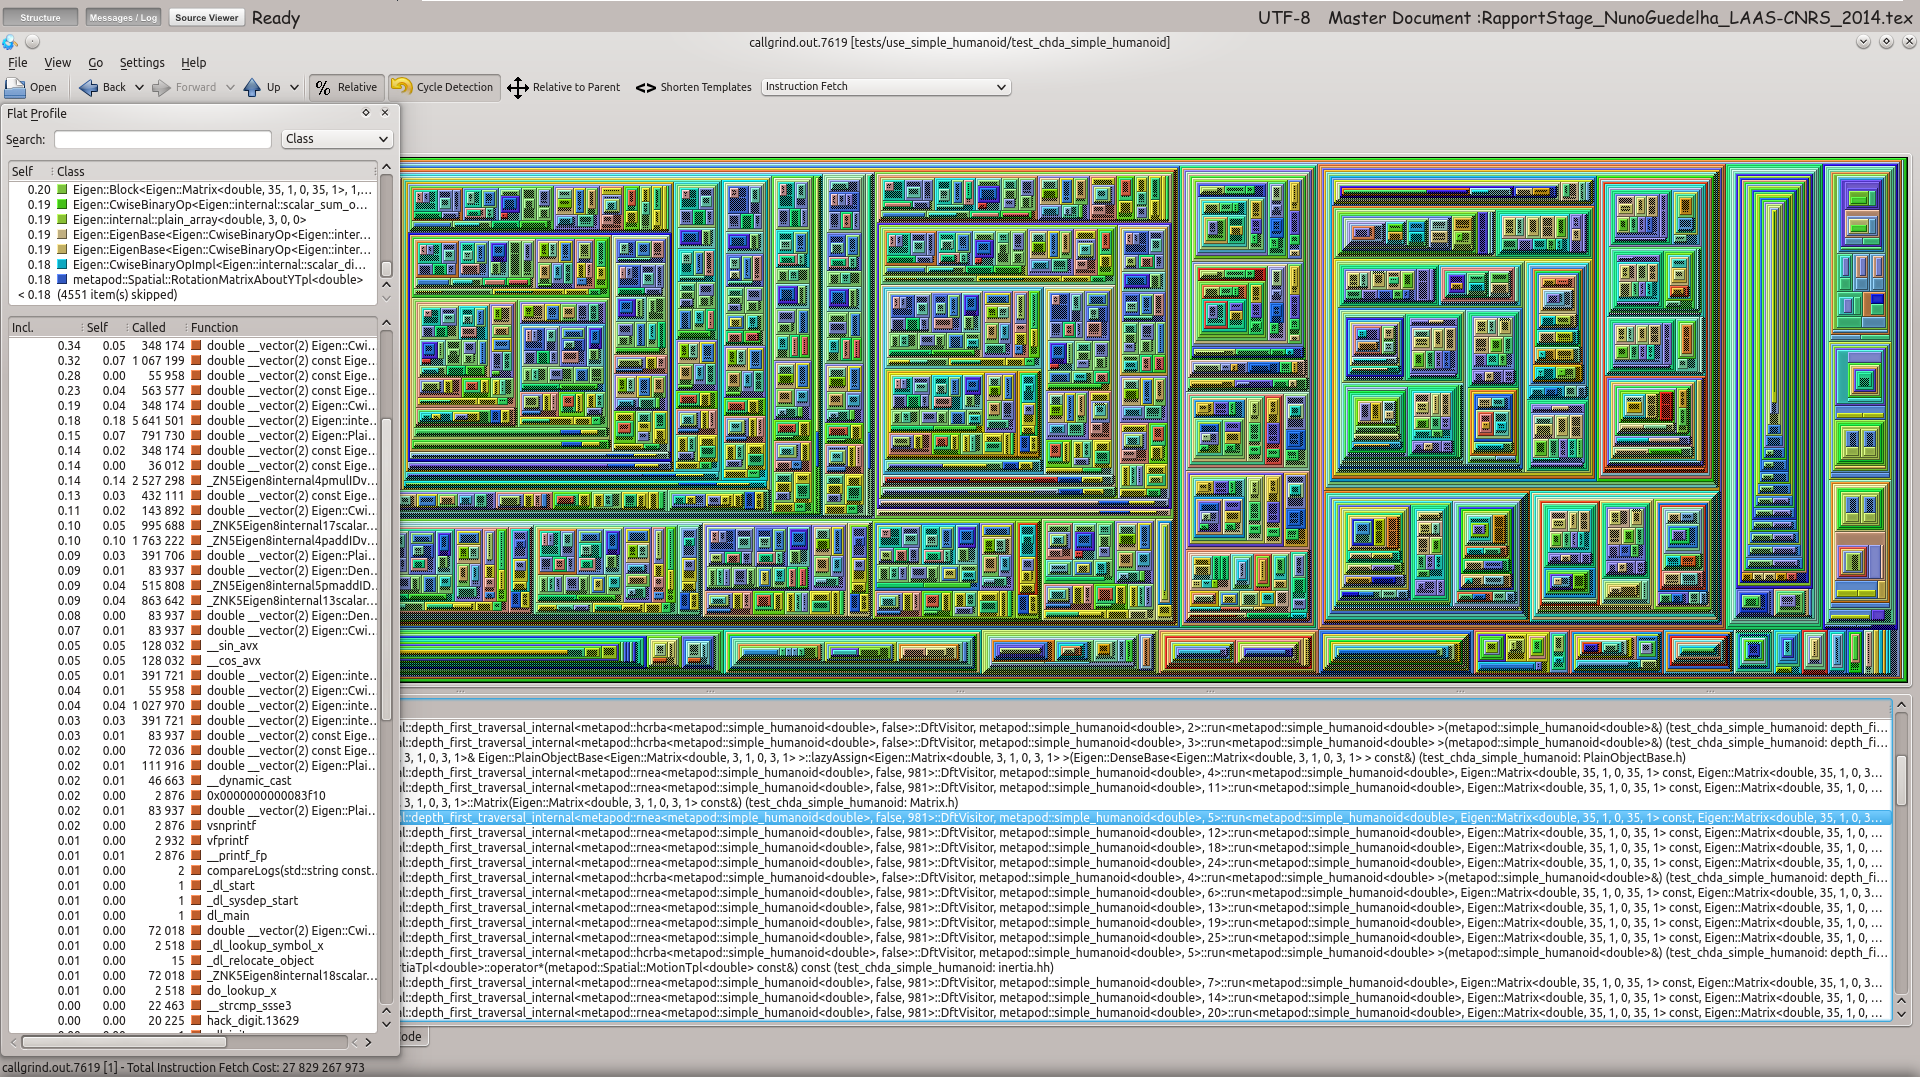
\includegraphics[width=\textwidth]{figs/snapshotKcachegrind1.png}
  \caption{Capture d'écran de Kcachegrind. Visualisation sous Kcachegrind du profil d'exécution des fonctions appelées par $test\_chda$.}         % legende
  \label{fig:Kcachegrind1} % pour citer le numéro de figure
  \end{center}
\end{figure}



\chapter{Concepts et théorèmes en mécanique du solide à la base de l'algèbre spatiale} \label{appx_torseursToalgSpa}

\section{Les torseurs} \label{appx_torseursToalgSpa_torseurs}

\setmyFiguresFile{torseurs}

\subsection{Définition} \label{appx_torseursToalgSpa_torseurs_def}
Les théorèmes généraux de la dynamique des systèmes matériels mettent en jeux deux ensembles de vecteurs liés: celui des quantités de mouvement (cinématique) et celui des forces (dynamique). Ces ensembles n'interviennent que par les torseurs qui leur sont associés. On appelle torseur ($T$) l'ensemble d'un champ antisymétrique $M(A)$ et de son vecteur $S$. $M(A)$ et $S$ sont appelés respectivement \emph{moment} et \emph{vecteur} du torseur $[T]$.

\vspace{0.3cm} % retour à la ligne

\minipages[2]{c}
{.3}{.7}{}
{%
\begin{equation*}
[\underline{T}]=
\begin{bmatrix}
  \underline{S} \\
  \underline{M}(O)
\end{bmatrix}
\end{equation*}
}
{%
\begin{equation}
M(A)=M(B)+AB \times S \textnormal{ ou } M(B)=M(A)+S \times AB
\end{equation}
}
{}

\vspace{0.3cm} % retour à la ligne

Le champ antisymétrique en question n'est pas forcément un champ de vecteurs liés. C'est le cas, par exemple, du torseur cinématique d'un corps rigide en mouvement, constitué à partir du champ antisymétrique des vitesses du solide (vitesse d'un point du solide coïncidant avec un point fixe de l'espace). nous développons ce point dans la section \ref{appx_torseursToalgSpa_torseurs_appl}.

\subsection{Propriétés} \label{appx_torseursToalgSpa_torseurs_prop}

Nous regroupons dans cette section les propriétés des torseurs qui sont directement héritées et utilisées en algèbre spatiale.

\begin{flushleft}
\begin{spacing}{1.5}
\begin{tabular}{ l l c p{5cm} }
  \textbf{\textsc{é}galité:}
  & $[T_{1}]=[T_{2}]$ & $\implies$ & $\mathbf{S}_{1}=\mathbf{S}_{2} \textnormal{ et } \mathbf{M}_{1}(A)=\mathbf{M}_{2}(A)$ \\
  \textbf{Somme:}
  & $[T]=[T_{1}]+[T_{2}]$ & $\implies$ & $\mathbf{S}=\mathbf{S}_{1}+\mathbf{S}_{2} \textnormal{ et } \mathbf{M}(A)=\mathbf{M}_{1}(A)+\mathbf{M}_{2}(A)$ \\
  \textbf{Multiplication par un scalaire:}
  & $[T_{1}]=\lambda [T_{2}]$ & $\implies$ & $\mathbf{S}_{1}=\lambda \mathbf{S}_{2} \textnormal{ et } \mathbf{M}_{1}(A)=\lambda \mathbf{M}_{2}(A)$ \\
  \textbf{Torseur nul:}
  & \multicolumn{3}{l}{$\mathbf{S}=0 \textnormal{ et } \mathbf{M}(A)=0$} \\
  \textbf{Produit scalaire:}
  & $si [F]={\mathbf{F},\mathbf{M}(A)} \textnormal{ et } [v]={\mathbf{w},\mathbf{V}(A)}$ & $\implies$ & $[F][v] = \mathbf{F} \cdot \mathbf{v}(A) + \mathbf{M}(A) \cdot \mathbf{w}$ \\
  \textbf{Invariants:}
  & \multicolumn{3}{l}{(équiprojectivité) la projection de $\mathbf{M}$ sur $\mathbf{S}$} \\
  & \multicolumn{3}{l}{(équiprojectivité) la projection de $\mathbf{M}$ sur $\mathbf{AB}$} \\
  & \multicolumn{3}{l}{Le produit scalaire $[F][v]$.} \\
  \multicolumn{1}{p{6cm}}{\textbf{Torseur lié à un ensemble de vecteurs liés:}}
  & \multicolumn{3}{p{10cm}}{Le moment d'un ensemble de vecteurs liés ${(A_{i},\mathbf{V}_{i})}$ a la forme d'un champ antisymétrique \cite{bib_champVecteurs} (chapitre IV). On lui associe donc
  le torseur} \\
  & \multicolumn{3}{l}{$\mathbf{S}=\Sigma_{i}\mathbf{V}_{i} (\emph{vecteur}) \textnormal{ et } \mathbf{M}(O)=\Sigma_{i}\mathbf{OA}_{i} \times \mathbf{V}_{i} (\emph{moment}).$} \\
\end{tabular}
\end{spacing}
\end{flushleft}

%Fixe la largeur de la 1ere colonne
%\newlength{\my1rstColumnWidth}
%\settowidth{\my1rstColumnWidth}{Multiplication par un scalaire:}
%\setlength{\my1rstColumnWidth}{.5in}

Remarque: on appelle invariants d'un torseur les quantités qui restent constantes quelque soit le point fixe dans l'espace où ce torseur est définit.

\subsection{applications} \label{appx_torseursToalgSpa_torseurs_appl}

\subparagraph{Torseur-vitesse:}

Dans l'étude de la dynamique des systèmes matériels, le champ de vitesses d'un corps rigide en mouvement \footnote{on se limite ici au cas des corps rigides} a la forme d'un champ antisymétrique (vecteurs non liés au corps), et son vecteur $\mathbf{w}$ définit la vitesse angulaire de rotation du solide. On lui associe donc un torseur dont les éléments de réduction sont:

\minipages[2]{|c}
{.75}{.4}{}
{%
\medskip
\begin{description}
  \item[vecteur $\mathbf{S}$:] vitesse angulaire $\mathbf{\omega}$ autour de l'axe de rotation considéré passant par $O$
  \item[moment $\mathbf{M}(O)$:] vitesse linéaire $\mathbf{v}(O)$ du solide au point $O$
\end{description}
\medskip
}{%
\\
\begin{tabular}{|r}
\(
\widehat{\underline{v}}_O=
\begin{bmatrix}
  \mathbf{\underline{S}}    \\
  \mathbf{\underline{M}}(O)
\end{bmatrix}
=
\begin{bmatrix}
  \mathbf{\underline{\omega}} \\
  \mathbf{\underline{v}}_O
\end{bmatrix}
\)
\end{tabular}
\medskip
}
{}

Et on peut exprimer la vitesse de deux points quelconques $A$ et $B$ liés au solide, par rapport à un repère fixe $R$, sous la forme:

\begin{equation}
\mathbf{v}_{B/\emph{R}}=\mathbf{v}_{A/\emph{R}}+\mathbf{BA} \times w_{S/\emph{R}}
\end{equation}
Nous retrouvons ici la forme de la vitesse spatiale établie dans la section \ref{algSpa_Vitesse}.

\subparagraph{Torseur cinétique:}

Le centre de masse $C$ d'un solide quelconque est défini par:
\begin{equation}
\mathbf{OC} = \frac{1}{M} \int_\vartheta \! \mathbf{OA}\rho \mathrm{d} \vartheta
\end{equation}
Où $\rho$ est la masse volumique, $\vartheta$ le volume total du corps rigide et $M$ sa masse totale. La quantité de mouvement $\mathbf{P}$ se calcule en intégrant les quantités de mouvement élémentaires $v \mathrm{d}m$ sur tout le volume $\vartheta$:
\begin{equation}
\mathbf{P} = \int_\vartheta \mathbf{v} \mathrm{d}m = \int_\vartheta \rho \mathbf{v} \mathrm{d}v = M\mathbf{v}_{C}
\end{equation}
De même, le moment cinétique $\mathbf{L}_{O}$ ($O$ origine d'un repère fixe dans l'espace) se calcule en intégrant les moments cinétiques élémentaires sur tout le volume $\vartheta$. Il en résulte une relation simple entre les moments cinétiques en $O$ et un autre point quelconque fixe de $\mathcal{R}$, $O'$:
\begin{equation}\label{momentKantiSym}
\mathbf{L}_O = \int_\vartheta \mathbf{OA} \times \mathbf{v}_A \rho \mathrm{d} \vartheta \quad \textnormal{ et } \quad \mathbf{L}_O = \mathbf{OO'} \times \mathbf{P} + \mathbf{L}_{O'}
\end{equation}
De plus, le théorème de Koenig permet de relier les moments cinétiques $\mathbf{L}_O$ par rapport à $\mathcal{R}$ et $\mathbf{L}^*$ par rapportà  $\mathcal{R^*}$, $\mathcal{R^*}$ étant le repère où le centre de masse est fixe. Le calcul de $\mathbf{L}_O$ dans $\mathcal{R}$ est ainsi simplifié:
\[
\begin{alignedat}{2}
\mathbf{L}_C = \mathbf{L}^* \quad \implies \quad \mathbf{L}_O = \mathbf{OC} \times \mathbf{P} + \mathbf{L}^* \quad \textnormal{ avec } &\quad \mathbf{L}^* &&= \int_\vartheta \rho \mathbf{CA} \times \mathbf{v}^* \mathrm{d} \vartheta \\
\textnormal{(Pour un solide)} &\quad \mathbf{L}^* &&= [I]_C \mathbf{\omega}
\end{alignedat}
\]

\textbf{Remarque:} Dans le cas d'un solide $\mathcal{S}$ en rotation ayant un point fixe $O$ dans $\mathcal{R}$, le moment cinétique exprimé en $O$ est donné par 
\colorbox[gray]{0.8}{\( \mathbf{L}_{O/\mathcal{R}} = [I]_O \mathbf{\omega} \)}, 
où $\mathbf{\omega}$ est le vecteur rotation du solide et $[I]_O$ est l'opérateur d'inertie dans $\mathcal{R}$. Or le centre de masse $C$ de $\mathcal{S}$ est bien un point fixe de $\mathcal{R^*}$, donc on obtient \colorbox[gray]{0.8}{\( \mathbf{L^*} = \mathbf{L}_{C/\mathcal{R^*}} = [I]_C \mathbf{\omega} \)}.

La relation entre les moments cinétiques en deux points fixes $O$ et $O'$ étant antisymétrique \eqref{momentKantiSym}, on peut associer au système de vecteurs liés $\{\rho \mathbf{v}_A \mathrm{d}\vartheta\}$, le torseur $[P]$ dit \emph{torseur cinétique}:

\minipages[2]{|c}
{.6}{.6}{}
{%
\medskip
\begin{description}
\item[moment $\mathbf{M}(O)$:] moment cinétique  $\mathbf{L}_O$ du solide au point $O$
\item[vecteur $\mathbf{S}$:] quantité de mouvement du système $\mathbf{P}$
\end{description}
\medskip
}{%
\\
\begin{tabular}{|r}
\(
\widehat{\underline{P}}_O=
\begin{bmatrix}
  \mathbf{\underline{M}}(O) \\
  \mathbf{\underline{S}}
\end{bmatrix}
=
\begin{bmatrix}
  \mathbf{\underline{\mathbf{L}}}_O \\
  \mathbf{\underline{P}}
\end{bmatrix}
\)
\end{tabular}
\medskip
}
{}


\subparagraph{Torseur-force:}

nous considérons maintenant les forces appliquées au solide $\mathcal{S}_d$ (déformable dans le cas général), toujours en mouvement par rapport au référentiel $\mathcal{R}$. Soit le vecteur lié générique $(A,\mathbf{f}_v)$ représentant la force volumique appliquée à l'élément de matière de volume $\mathrm{d}\vartheta$ qui entoure $A$, un point fixe de $\mathcal{S}$ (figure \ref{fig_systemeDeForces.a}. Cette force inclut les forces extérieures à $\mathcal{S}_d$ ainsi que les forces exercées par les autres éléments de matière de $\mathcal{S}_d$. Notamment, si le référentiel n'est pas galiléen, il faut compter également les forces de Coréolis. On représente donc le système de forces appliquées à $\mathcal{S}_d$ par l'ensemble des vecteurs liés ${(A,\mathbf{f}_v\mathrm{d}\vartheta)}$, pour lequel on calcule la somme des forces et le moment (couple) résultant des forces $O$:

\begin{equation}
\mathbf{f} = \int_\vartheta \mathbf{f}_v\mathrm{d}\vartheta \textnormal{ et } \mathbf{n}_O = \int_\vartheta \mathbf{OA} \times \mathbf{f}_v\mathrm{d}\vartheta
\end{equation}

\dispThreeFig[H]
{1}{vecteur force volumique lié}
{2}{somme des forces et moment des forces}
{3}{Transformation: moment par rapport à un autre point $O'$}
{système de forces des vecteurs liés ${(A,\mathbf{f}_v\mathrm{d}\vartheta)}$}
{fig_systemeDeForces}

Dans cette représentation, on considère $S$ comme une force linéaire globale passant par $O$, avec son moment global $M$ en $O$ associé (figure \ref{fig_systemeDeForces.b}).
On calcule également la relation simple entre les moments des forces en $O$ et un autre point quelconque fixe de $\mathcal{R}$, $O'$ (figure \ref{fig_systemeDeForces.c}):
\begin{equation}\label{}
\mathbf{n}_O = \int_\vartheta (\mathbf{OO'} + \mathbf{O'A}) \times \mathbf{f}_v\mathrm{d}\vartheta = \mathbf{n}_{O'} + \mathbf{OO'} \times \mathbf{f}
\end{equation}

On peut donc associer au système de vecteurs liés ${(A,\mathbf{f}_v\mathrm{d}\vartheta)}$ le torseur $[F]$ dit \emph{torseur-force}:

\minipages[2]{|c}
{.7}{.6}{}
{%
\medskip
\begin{description}
\item[moment $\mathbf{M}(O)$:] couple résultant des forces $\mathbf{n}_O$ du solide au point $O$
\item[vecteur $\mathbf{S}$:] somme des forces du système $\mathbf{f}$
\end{description}
\medskip
}{%
\\
\begin{tabular}{|r}
\(
\widehat{\underline{f}}_O=
\begin{bmatrix}
  \mathbf{\underline{M}}(O) \\
  \mathbf{\underline{S}}
\end{bmatrix}
=
\begin{bmatrix}
  \mathbf{\underline{\mathbf{n}}}_O \\
  \mathbf{\underline{f}}
\end{bmatrix}
\)
\end{tabular}
\medskip
}
{}

Remarque: Les torseurs $\widehat{f}_O$ et $\widehat{f}_O'$ sont équivalents car ils décrivent les mêmes force/mouvement du centre de masse et couple autour du centre de masse du solide. Cette équivalence n'est pas forcément vraie pour l'ensemble du système de forces (par exemple le cas d'un ressort soit comprimé soit étiré par deux forces parallèles et opposées).


\subparagraph{Torseur dynamique:}

Comme pour la quantité de mouvement $P$ et le moment cinétique $L$, nous calculons la quantité d'accélération (somme dynamique) et le moment résultant de cette accélération (moment dynamique) en intégrant les grandeurs élémentaires respectives sur tout le volume, et nous montrons que:
\begin{align}
\mathbf{D} &= \int_\vartheta \mathbf{a} \mathrm{d}m = \frac{\mathrm{d}}{\mathrm{d}t} \int_\vartheta \mathbf{v} \mathrm{d}m = \frac{\mathrm{d}}{\mathrm{d}t} (M \mathbf{v}_{C}) \\
\mathbf{L}_O &= \int_\vartheta \mathbf{OA} \times \rho \mathbf{a}_A \mathrm{d} \vartheta \quad \textnormal{ et } \quad \mathbf{N}_O = \mathbf{OO'} \times \mathbf{D} + \mathbf{N}_{O'}
\end{align}
où $O'$ est un autre point fixe de $\mathcal{R}$.

\medskip

On peut donc associer au système de vecteurs liés ${(A,\rho \mathbf{a}_A \mathrm{d}\vartheta)}$ le torseur $[D]$ dit \emph{torseur dynamique}:

\minipages[2]{|c}
{.7}{.6}{}
{%
\medskip
\begin{description}
\item[moment $\mathbf{M}(O)$:] moment dynamique résultant $\mathbf{N}_O$ du solide au point $O$
\item[vecteur $\mathbf{S}$:] quantité d'accélération du centre de masse $\mathbf{D}$
\end{description}
\medskip
}{%
\\
\begin{tabular}{|r}
\(
\widehat{\underline{D}}_O=
\begin{bmatrix}
  \mathbf{\underline{M}}(O) \\
  \mathbf{\underline{S}}
\end{bmatrix}
=
\begin{bmatrix}
  \mathbf{\underline{\mathbf{N}}}_O \\
  \mathbf{\underline{D}}
\end{bmatrix}
\)
\end{tabular}
\medskip
}
{}



\chapter{Quelques démonstrations en algèbre spatiale} \label{appx_dem}

\setmyFiguresFile{figures}

\section{Invariance du vecteur spacial $\widehat{v}$}

Si on définit deux bases de \emph{Plücker} différentes $D_{O}$ et $D_{P}$, centrées respectivement sur $O$ et $P$:

\begin{align*}
D_{O} = \lbrace &\textbf{d}_{Ox}, \textbf{d}_{Oy}, \textbf{d}_{Oy}, \textbf{d}_{x}, \textbf{d}_{y}, \textbf{d}_{z} \rbrace \\
D_{P} = \lbrace &\textbf{d}_{Px}, \textbf{d}_{Py}, \textbf{d}_{Py}, \textbf{d}_{x}, \textbf{d}_{y}, \textbf{d}_{z} \rbrace \\
\end{align*}

Ainsi que les vecteurs spatiaux associés $\widehat{v}$ et $\widehat{v'}$, on obtient:

\begin{align}
\widehat{v}  &= \underline{v}_{O} \cdot D_{O} \notag \\
\widehat{v'} &= \underline{v}_{P} \cdot D_{P} \notag \\
^{D_{O}}\widehat{v} \quad &= \quad ^{D_{O}}\widehat{v'}
\label{equ_invariant}
\end{align}


Les projections de ces deux vecteurs spatiaux $\widehat{v}$ et $\widehat{v'}$ dans la même base de \emph{Plücker} sont identiques \eqref{equ_invariant}. Il faut noter que si les deux bases ont la même orientation, elles auront les mêmes vecteurs unitaires de translation ($\textbf{d}_{x}$, $\textbf{d}_{y}$ et $\textbf{d}_{z}$), mais les vecteurs unitaires de rotations diffèrent si $O \neq P$ ne sont pas confondus, comme illustré dans le l'exemple de cas simple ci-dessous:

\dispThreeFig[H]
{4}{Deux bases de \emph{Plücker} de même orientation.}
{5}{Expression de $\textbf{d}_{Py}$ et $\textbf{d}_{Pz}$ en $O$.}
{6}{cas de $\textbf{d}_{Pz}$ (projection suivant $\textbf{d}_{z}$).}
{Expression de $\textbf{d}_{Px}$, $\textbf{d}_{Py}$ et $\textbf{d}_{Pz}$ en $O$.}
{vitessePointCoincidant}


Pour rapidement comprendre ces transformations, on peut visualiser un corps tournant autour de l'axe $P_{y}$ à la vitesse $w_{y}$. On définit initialement le vecteur spatial $\widehat{v'}$ en $P$ (\cad considérant l'axe de rotation du corps autour de $P_{y}$) est alors $w_{y}\textbf{d}_{Py}$. Or la vitesse d'un point lié au corps et passant par $O$ (par rapport au repère fixe $R(O,x,y,z)$) vaut $rw_{y}\textbf{d}_{z}$. Le vecteur spatial en $O$ (\cad considérant le corps en rotation autour de l'axe $O_{y}$) est alors $\widehat{v}=\textbf{d}_{Oy}+r\textbf{d}_{z}$. Nous montrons ainsi, pour tous les axes, que:

\begin{align*}
  \textbf{d}_{Px} &= \textbf{d}_{Ox} \\
  \textbf{d}_{Py} &= \textbf{d}_{Oy}+r \textbf{d}_{z} \\
  \textbf{d}_{Pz} &= \textbf{d}_{Oz}-r \textbf{d}_{y}
\end{align*}

On considère à présent un corps $C$ en translation et en rotation autour d'un axe quelconque dans l'espace. Le vecteur spatial $\widehat{v}$ de ce corps en $O$, s'exprime dans la base de \emph{Plücker} $D_{O}$ comme suit:

\begin{equation*}
  \widehat{v} = w_{x}\textbf{d}_{Ox} + w_{y}\textbf{d}_{Oy} + w_{z}\textbf{d}_{Oz} + v_{Ox}\textbf{d}_{x} + v_{Oy}\textbf{d}_{y} + v_{Oz}\textbf{d}_{z}
\end{equation*}

Le vecteur spatial $\widehat{v'}$ de ce corps en $P$, s'exprime dans la base de \emph{Plücker} $D_{P}$ comme suit:

\begin{equation*}
  \widehat{v'} = w_{x}\textbf{d}_{Px} + w_{y}\textbf{d}_{Py} + w_{z}\textbf{d}_{Pz} + v_{Px}\textbf{d}_{x} + v_{Py}\textbf{d}_{y} + v_{Pz}\textbf{d}_{z}
\end{equation*}

Nous voulons l'exprimer dans la base $D_{O}$. $w_{x}$, $w_{y}$ et $w_{z}$ sont connus. Calculons $v_{Px}$, $v_{Py}$ et $v_{Pz}$:

\vspace{0.3cm}
\minipages[2]{t}{.4}{.6}{}
{%
\(
\begin{alignedat}{3}
  & &&\phantom{xxx} v_{P} &&= v_{O} + w \times \overrightarrow{OP} \\
  \vspace{0.5cm}
  &\iff &&\phantom{xxx} \underline{v}_{P}
  &&=
  \underline{v}_{O}+\underline{w}\times
  \begin{bmatrix}
    r\\
    0\\
    0
  \end{bmatrix} \\
  \vspace{0.5cm}
  &\iff
  &&\begin{bmatrix}
    v_{Px} \\
    v_{Py} \\
    v_{Pz}
  \end{bmatrix}
  &&=
  \begin{bmatrix}
    v_{Ox}\\
    v_{Oy}+w_{z}r\\
    v_{Oz}-w_{y}r
  \end{bmatrix}
  \quad \texttt{or} \quad
  \widehat{\underline{v}'}
  =
  \begin{bmatrix}
    \underline{w} \\
    \underline{v}_{P}
  \end{bmatrix}
\end{alignedat}
\)}
{%
\begin{tabular}{|p{\textwidth}}
\(\begin{alignedat}{2}
  &\iff
  \widehat{v'} &&= w_{x}\textbf{d}_{Px} + w_{y}\textbf{d}_{Py} + w_{z}\textbf{d}_{Pz} \\
  &            &&\phantom{{}={}} + v_{Px}\textbf{d}_{x} + v_{Py}\textbf{d}_{y} + v_{Pz}\textbf{d}_{z} \\
  &            &&= w_{x}\textbf{d}_{Ox} + w_{y}(\textbf{d}_{Oy}+r\textbf{d}_{z}) + w_{z}(\textbf{d}_{Oz}-r\textbf{d}_{y}) \\
  &            &&\phantom{{}={}} + v_{Ox}\textbf{d}_{x} + (v_{Oy}+w_{z}r)\textbf{d}_{y} + (v_{Oz}-w_{y}r)\textbf{d}_{z} \\
  &            &&= w_{x}\textbf{d}_{Ox} + w_{y}\textbf{d}_{Oy} + w_{z}\textbf{d}_{Oz} + v_{Ox}\textbf{d}_{x} + v_{Oy}\textbf{d}_{y} + v_{Oz}\textbf{d}_{z} \\
  &            &&= \widehat{v}
\end{alignedat}\)
\end{tabular}
}
{}
\vspace{0.3cm}

Nous avons ainsi montré l'équivalence des deux vecturs spatiaux $\widehat{v}$ et $\widehat{v'}$.

La propriété d'invariance se vérifie pour tout point $O$ et $P$ fixes dans l'espace et une orientation quelconque des repères $R(O,x,y,z)$ et $R'(P,x,y,z)$. Nous pouvons trouver la démonstration complète de cette propriété d'invariance dans l'annexe \ref{appx_dem}.










% Bibliography:
\clearpage
\addcontentsline{toc}{chapter}{Bibliography}

\begin{thebibliography}{9}

\bibitem{bib_featherstone}
  Roy Featherstone,
  \emph{Rigid Body Dynamics Algorithms}.
  Springer Science+Business Media, LLC,
  $2^{nd}$ edition,
  2008.

\bibitem{bib_torseur}
  E. Ramis, C. Deschamps et J. Odoux,
  \emph{Algèbre et applications à la géométrie}.
  Masson, coll. "Cours de mathématiques spéciales"
  $2^{edition}$, 1987 (ISBN 2-225-63404-1),
  chap. 8 ("Les torseurs"), p. 276-294
  
\bibitem{bib_champVecteurs}
  José-Philippe Pérez,
  \emph{Mécanique, Fondements et applications}.
  Masson Sciences,
  $6^{e}$ édition, 2001 (ISBN 2-10-005464-3),
  chap. 1 ("Calcul vectoriel. Torseurs") - section IV, V et VI - p. 8-15, 
  chap. 16 (Cinématique du solide et des solides en contact) - section I - p. 257, 295
  
\bibitem{bib_eigen_tutorial_alg_lin}
  Eigen - Tutorial Linear Algebra:
  http://eigen.tuxfamily.org/dox/%group__TutorialLinearAlgebra.html
  
\bibitem{bib_eigen_tutorial_catalogue}
  Eigen - Catalogue of dense decompositions,
  %http://eigen.tuxfamily.org/dox/group__TopicLinearAlgebraDecompositions.html
  
\bibitem{bib_eigen_LLT_desc}
  Eigen - LLT detailed description,
  %http://eigen.tuxfamily.org/dox/classEigen_1_1LLT.html

\bibitem{bib_eigen_tutorial_catalogue_sparse}
  Eigen - Solving Sparse Linear Systems
  %http://eigen.tuxfamily.org/dox/group__TopicSparseSystems.html

\bibitem{bib_ros}
  ROS - site internet:
  http://wiki.ros.org/urdf/

\bibitem{bib_urdf}
  URDF - page internet sous le site ROS:
  http://wiki.ros.org/urdf/

%\bibitem{bib_matriceDefiniePositive_1}
%Horn & Johnson (1985), p. 397

%\bibitem{bib_matriceDefiniePositive_2}
%http://en.wikipedia.org/wiki/Positive-definite_matrix

%\bibitem{bib_openMPcompilers}
%  "OpenMP Compilers"at OpenMP.org,
%  http://openmp.org/wp/openmp-compilers/
%  2013-04-10. Retrieved 2013-08-14.

\bibitem{bib_openMPspecs}
  The OpenMP API specification for parallel programming,
  http://openmp.org/wp/openmp-specifications/

\bibitem{bib_openMpWikipedia}
  http://en.wikipedia.org/wiki/OpenMP
  
\bibitem{bib_decompositionLUwikipedia}
  Wikipedia% - Décomposition LU
%  http://fr.wikipedia.org/wiki/Décomposition_LU

\bibitem{bib_decompositionLU_1}
  Cours d'analyse numérique de licence (2010) de R. Herbin, Université d'Aix-Marseille, section 1.3.1, pages 25-26
  http://www.cmi.univ-mrs.fr/~herbin/PUBLI/anamat.pdf
  
\bibitem{bib_decompositionLU_2}
  P. G. Ciarlet - « Introduction à l'analyse numérique matricielle et à l'optimisation » (1985, rééd. 2001), éd. Masson, coll. Math. Appl. pour la Maîtrise (ISBN 2-225-68893-1)

%\bibitem{bib_complexiteInversionMatriceDirecte}
%  SUR L'INVERSION DE MATRICE,
  J.B Lasserre,
%  http://archive.numdam.org/ARCHIVE/RO/RO_1992__26_2/RO_1992__26_2_177_0/RO_1992__26_2_177_0.pdf

\end{thebibliography}



\end{document}
